\documentclass{sigchi}

% Use this section to set the ACM copyright statement (e.g. for
% preprints).  Consult the conference website for the camera-ready
% copyright statement.

% Copyright
\CopyrightYear{2016}
%\setcopyright{acmcopyright}
\setcopyright{acmlicensed}
%\setcopyright{rightsretained}
%\setcopyright{usgov}
%\setcopyright{usgovmixed}
%\setcopyright{cagov}
%\setcopyright{cagovmixed}
% DOI
\doi{http://dx.doi.org/10.475/123_4}
% ISBN
\isbn{123-4567-24-567/08/06}
%Conference
\conferenceinfo{CHI'16,}{May 07--12, 2016, San Jose, CA, USA}
%Price
\acmPrice{\$15.00}

% Use this command to override the default ACM copyright statement
% (e.g. for preprints).  Consult the conference website for the
% camera-ready copyright statement.

%% HOW TO OVERRIDE THE DEFAULT COPYRIGHT STRIP --
%% Please note you need to make sure the copy for your specific
%% license is used here!
% \toappear{
% Permission to make digital or hard copies of all or part of this work
% for personal or classroom use is granted without fee provided that
% copies are not made or distributed for profit or commercial advantage
% and that copies bear this notice and the full citation on the first
% page. Copyrights for components of this work owned by others than ACM
% must be honored. Abstracting with credit is permitted. To copy
% otherwise, or republish, to post on servers or to redistribute to
% lists, requires prior specific permission and/or a fee. Request
% permissions from \href{mailto:Permissions@acm.org}{Permissions@acm.org}. \\
% \emph{CHI '16},  May 07--12, 2016, San Jose, CA, USA \\
% ACM xxx-x-xxxx-xxxx-x/xx/xx\ldots \$15.00 \\
% DOI: \url{http://dx.doi.org/xx.xxxx/xxxxxxx.xxxxxxx}
% }

% Arabic page numbers for submission.  Remove this line to eliminate
% page numbers for the camera ready copy
% \pagenumbering{arabic}

% Load basic packages
\usepackage{balance}       % to better equalize the last page
\usepackage{graphics}      % for EPS, load graphicx instead 
\usepackage[T1]{fontenc}   % for umlauts and other diaeresis
\usepackage{txfonts}
\usepackage{mathptmx}
\usepackage[pdflang={en-US},pdftex]{hyperref}
\usepackage{color}
\usepackage{booktabs}
\usepackage{textcomp}
\usepackage{multirow}
\usepackage{caption}
\usepackage{subcaption}

% Some optional stuff you might like/need.
\usepackage{microtype}        % Improved Tracking and Kerning
% \usepackage[all]{hypcap}    % Fixes bug in hyperref caption linking
\usepackage{ccicons}          % Cite your images correctly!
% \usepackage[utf8]{inputenc} % for a UTF8 editor only

% If you want to use todo notes, marginpars etc. during creation of
% your draft document, you have to enable the "chi_draft" option for
% the document class. To do this, change the very first line to:
% "\documentclass[chi_draft]{sigchi}". You can then place todo notes
% by using the "\todo{...}"  command. Make sure to disable the draft
% option again before submitting your final document.
\usepackage{todonotes}

% Paper metadata (use plain text, for PDF inclusion and later
% re-using, if desired).  Use \emtpyauthor when submitting for review
% so you remain anonymous.
\def\plaintitle{Bike Angels: An Analysis of Citi Bike's Incentive Program}
\def\plainauthor{First Author, Second Author, Third Author,
  Fourth Author, Fifth Author, Sixth Author}
\def\emptyauthor{}
\def\plainkeywords{Authors' choice; of terms; separated; by
  semicolons; include commas, within terms only; required.}
\def\plaingeneralterms{Documentation, Standardization}

% llt: Define a global style for URLs, rather that the default one
\makeatletter
\def\url@leostyle{%
  \@ifundefined{selectfont}{
    \def\UrlFont{\sf}
  }{
    \def\UrlFont{\small\bf\ttfamily}
  }}
\makeatother
\urlstyle{leo}

% To make various LaTeX processors do the right thing with page size.
\def\pprw{8.5in}
\def\pprh{11in}
\special{papersize=\pprw,\pprh}
\setlength{\paperwidth}{\pprw}
\setlength{\paperheight}{\pprh}
\setlength{\pdfpagewidth}{\pprw}
\setlength{\pdfpageheight}{\pprh}

% Make sure hyperref comes last of your loaded packages, to give it a
% fighting chance of not being over-written, since its job is to
% redefine many LaTeX commands.
\definecolor{linkColor}{RGB}{6,125,233}
\hypersetup{%
  pdftitle={\plaintitle},
% Use \plainauthor for final version.
%  pdfauthor={\plainauthor},
  pdfauthor={\emptyauthor},
  pdfkeywords={\plainkeywords},
  pdfdisplaydoctitle=true, % For Accessibility
  bookmarksnumbered,
  pdfstartview={FitH},
  colorlinks,
  citecolor=black,
  filecolor=black,
  linkcolor=black,
  urlcolor=linkColor,
  breaklinks=true,
  hypertexnames=false
}

% create a shortcut to typeset table headings
% \newcommand\tabhead[1]{\small\textbf{#1}}

% End of preamble. Here it comes the document.
\begin{document}

\title{\plaintitle}

\numberofauthors{3}
\author{%
  \alignauthor{Leave Authors Anonymous\\
    \affaddr{for Submission}\\
    \affaddr{City, Country}\\
    \email{e-mail address}}\\
  \alignauthor{Leave Authors Anonymous\\
    \affaddr{for Submission}\\
    \affaddr{City, Country}\\
    \email{e-mail address}}\\
  \alignauthor{Leave Authors Anonymous\\
    \affaddr{for Submission}\\
    \affaddr{City, Country}\\
    \email{e-mail address}}\\
}

\maketitle


\begin{abstract}
Bike-sharing systems provide a sustainable and affordable transportation alternative in many American cities. However, they also face intricate challenges due to imbalance, caused by asymmetric traffic demand. That imbalance often-times leads to bike-sharing stations being empty (full), causing out-of-stock events for customers that want to rent (return) bikes at such stations. In recent years, the study of data-driven methods to help support the operation of such system, has developed as a popular research area. 

In this paper, we study the impact of \emph{Bike Angels}, an incentive program New York City's Citi Bike system set up in 2015 to crowdsource some of its operational challenges related to imbalance. We develop a performance metric for both online- and offline-policies to set incentives within the system; our results indicate that though Citi Bike's original offline policy performed well in a regime in which incentives given to customers are not associated to costs, there is ample space for improvement when the costs of the incentives are taken into consideration. Motivated by these findings, we develop several online- and offline- policies to investigate the trade-offs between real-time and offline decision-making; one of our online policies has since been adopted by Citi Bike.
%The largest American bike-sharing system, Citi Bike operated by New York City Bikeshare, set up their \emph{Bike Angels} program in 2015. In this work, we study its impact on system imbalance. As \emph{Bike Angels} was initiated with offline decision-making, i.e., by setting incentives ahead of time without knowledge of the system state, the incentives were not always efficient from a rebalancing perspective. Our work quantifies the impact of the offline scheme and investigates the trade-offs required between offline and online decision making in this context by estimating the efficiency of a range of different offline and online policies. 

%On-demand transportation systems, like ride-sharing, bike-sharing, and car-sharing, have evolved as an important application of modern data science techniques. In all of these, platforms apply operational levers to reduce the system imbalance caused by asymmetric traffic flows. This is often referred to as \emph{rebalancing}. The large scale of these systems inherently requires quantitative support to rebalance efficiently. Recently, bike-sharing systems have introduced incentive schemes to crowd-source the operational challenges. The largest American bike-sharing system, Citi Bike operated by New York City Bikeshare, set up their \emph{Bike Angels} program in 2015. In this work, we study its impact on system imbalance. As \emph{Bike Angels} was initiated with offline decision-making, i.e., by setting incentives ahead of time without knowledge of the system state, the incentives were not always efficient from a rebalancing perspective. Our work quantifies the impact of the offline scheme and investigates the trade-offs required between offline and online decision making in this context by estimating the efficiency of a range of different offline and online policies. 
\end{abstract}

%
% The code below should be generated by the tool at
% http://dl.acm.org/ccs.cfm
% Please copy and paste the code instead of the example below.
%
\begin{CCSXML}
<ccs2012>
 <concept>
  <concept_id>10010520.10010553.10010562</concept_id>
  <concept_desc>Information systems~Crowdsourcing~Incentive schemes</concept_desc>
  <concept_significance>300</concept_significance>
 </concept>
  <concept>
  <concept_id>10010520.10010553.10010562</concept_id>
  <concept_desc>Applied Computing~Transportation</concept_desc>
  <concept_significance>300</concept_significance>
 </concept>
</ccs2012>
\end{CCSXML}

\ccsdesc[500]{Information systems ~ Incentive schemes}
\ccsdesc[300]{Applied Computing ~ Transportation}
%\ccsdesc{Computer systems organization~Robotics}
%\ccsdesc[100]{Networks~Network reliability}


\keywords{Sustainable Transportation, Crowdsourcing, Bikesharing, Incentives, Inventory Management}


\maketitle

\section{Introduction}
%TODO One paragraph (3 sentences) on bikesharing having become ubiquitous, NYC being the largest systems in the US and rebalancing being the major operational challenge. Explain that full stations stop customers from returning, empty stations from renting -- both suck.
Bike-sharing systems have become ubiquitous in many American cities. The largest of these systems consist of a number of stations placed densely within a city; each station consists of a number of docks that each either hold a bike (are full) or are empty. Users can rent a bike from any station with at least one bike and return bikes at any station with an empty dock. With more than 30 million annual rides nationwide (2017), about half of which occurred in New York City's Citi Bike system, these systems have become a fixture of urban life, providing commuters and tourists with a sustainable transportation option.

The major operational challenge faced by these systems is to avoid out-of-stock events: as each station has a finite number of docks (\emph{capacity}) at which users can rent or return bikes, users are unable to enter the system when trying to rent bikes at stations at which all docks are empty, that is, when no dock holds a bike; arguably even worse, customers are not able to leave the system when they try to return bikes at stations at which all docks are full. In the past few years, researchers and system operators alike have developed tools to tackle such out-of-stock events and their underlying cause: \emph{imbalance}. This is often referred to as \emph{rebalancing}: moving bikes within the system to reduce the number of out-of-stock events. Rebalancing can be of various modes: for example, systems operate box trucks, pedicab trailers, and valet services to reduce out-of-stock events. In this paper, we describe our work with the operators of Citi Bike in setting up \emph{Bike Angels}, a crowdsourcing approach to rebalancing, and analyze the relative effectiveness of a variety of natural incentive schemes for their system.

The Bike Angels incentive scheme was first set up in October 2015. In the initial set-up, we identified pairs of stations that (i) were close to each other, and (ii) had asymmetric demand patterns: we chose pairs of stations that were nearby to each other but over a certain time interval had the property that one station (A) overwhelmingly had bikes returned whereas the other (B) overwhelmingly had bikes rented. We then invited users that often used one of the two and asked them to switch to the other, i.e., we asked a small number of customers likely to return bikes at A in such intervals to become \emph{Bike Angels} by instead returning bikes at~B. Of course, in such a scheme, incentives can only be used for a tiny fraction of rides within the system.

Nevertheless, the pilot showed that customer behavior could be significantly affected through gamification \cite{citibikeInternal}, and also posed questions about how to optimally design such an incentive scheme, in particular with respect to when and where to incentivize. A second version of Bike Angels, at a much larger scale, statically incentivized a sizeable fraction of stations within the system either to enourage rentals or returns throughout each rush hour.
This program was viewed as a great success, in spite of the fact that the pre-determined incentives made no use of the vast amounts of historic and real-time data available. At worst, this sometimes led to incentives  encouraging customers to rent (return) bikes at empty (full) stations. % about which station is labeled as what were made long ahead of time, we could not guarantee that stations that are usually in need of bikes at particular times would not end up full at those times (or vice-versa for stations usually overfilled with bikes).

In this paper, we evaluate the efficiency of this incentive scheme with regard to its goal to reduce out-of-stock events.  We apply so-called \emph{user dissatisfaction functions} to evaluate, for every trip rewarded by the program, an estimate of its reduction in future out-of-stock events. Further, we design a range of different policies, dictating the times at which each station is incentivized. The design of these policies involves trade-offs between their \emph{efficiency} and \emph{simplicity}. Below, we explain what we mean by those two terms:

\noindent \textbf{Efficiency.} The main goal of \emph{Bike Angels} is to help rebalance the system, i.e., to reduce the number of out-of-stock events. We explain in subsequent sections how the user dissatisfaction functions introduced by Raviv and Kolka  \cite{raviv2013optimal} can be used to evaluate the impact of each individual rental/return on the expected number of future out-of-stock events. Combining these with a cost for each point awarded in the incentive scheme, we obtain a score for each incentivized rental/return that can be interpreted as an offline evaluation of the efficiency of the incentive. In that sense, a perfectly efficient scheme would incentivize exactly those trips that net a positive score when accounting for both the impact on out-of-stock events and the cost of incentives.

\noindent \textbf{Simplicity. } Perfect efficiency, with respect to the score described above, is attainable in such an incentive scheme, but it requires the operator to decide in real-time whether or not to incentivize at each location. This is undesirable from the users' perspective as it reduces predictability on where incentives will be given in the future, i.e., when customers prepare their trip, they do not know whether or not their origin and, even more so, their destination has rentals and respectively, returns, incentivized. This raises the bar for participation. Further, from an operator's perspective, the IT set-up for a dynamic scheme requires more maintenance than, say, the completely static version. %Very dynamic is bad for customer experience, predictability is useful, if we know ahead of time where incentives are happening, that makes it more convenient for users as it means that (1) they don't need to check the app if they know and (2) they are guaranteed ahead of time whether or not their trip will give points

We show that even though there exist natural trade-offs between the two, there are a variety of incentive policies that span the continuum from maximally efficient and maximally dynamic to less efficient and entirely static. Our results employ a data-driven methodology to design such policies, one of which is now in place at Citi Bike.


\subsection{Related Work}\label{sec:rel_work}

Our analysis is a novel application of the user dissatisfaction functions defined by \cite{raviv2013optimal} which provide a mathematical framework to characterize the expected number of out-of-stock events in the system over a specified planning period. Different ways to compute these user dissastisfaction functions were subsequently suggested \cite{schuijbroek2013inventory,henomashm16,parikh2014estimation}. Each of these relies on demand estimates at each station, which we obtain through the decensoring method suggested in \cite{o2015data}. Within the literature on operations in bikesharing systems, these user dissatisfaction functions have usually been used in routing problems, see \cite{raviv2013static,forma20153,ho2014solving,szeto2016chemical,Freund2016Rebalancing} among others. Additionally, they have also been successfully applied in the context of system design, that is, to analyse the number of docks that should be placed at every location within a system \cite{henomashm16, frehenshm17}.

An incentive scheme like the one we study here was first suggested for bikehsaring schemes by \cite{henomashm16}; in other transportation settings, a similar scheme was succesfully implemented by \cite{merugu2009incentive}. In contrast, while the work by \cite{singla2015incentivizing} also studies an incentive scheme for bikesharing, that work focuses on how much to incentivize to ensure people act upon it, rather than on the effects of incentivized trips on the balance of the system.

In the queueing literature, on-demand transportation systems have been investigated under steady-state regimes with approaches to incentives being studied by \cite{fricker2012incentives,fricker2016incentives}. This also has relations to pricing questions in ridesharing systems as studied by \cite{george2012stochastic,Waserhole2014,banerjee2017pricing}. The steady-state assumption, however, is difficult to justify in bikesharing systems, given that (i) most of the traffic occurs during rush hours and (ii) the configuration of bikes within the system vastly differs at the beginning and end of each rush hour. Despite the steady-state assumption being hard to justify, it is worth highlighting a parallel to \cite{banerjee2015pricing} who study the trade-offs between dynamic and static pricing policies in ride-sharing systems. Similar such trade-offs were more recently studied by \cite{chen2017pricing}. Though these works consider very different models, they consider the same trade-offs as we do in the context of modern transportation systems. %their main theorem parallels our result in Section \ref{ssec:theorem} which shows that in appropriate fluid settings, static policies achieve optimal performance.


%\subsection{Contribution}\label{sec:contribution}
%
%We develop a data-driven approach to evaluate the trade-offs necessary between different possible incentive policies. To that effect, our contribution is threefold:
%
%\begin{enumerate}
%\setlength\itemsep{-.3em} 
%    \item We apply the inventory model defined by \cite{raviv2013optimal} to define a performance metric for Citi Bike's incentive scheme; using the inventory model and data collected through CitiBike's \emph{Bike Angel} program we estimate for every ride rewarded by the incentive scheme the impact on dissatisfied users.
%    \item We design several policies to decide when to incentivize at each station.
%    \item Using the performance metric, we evaluate the different policies, and study the trade-offs between their simplicity and performance.
%\end{enumerate}
%
%Though many papers in recent years have theoretically investigated the trade-offs between static/offline and dynamic/online decision-making associated to transportation in the sharing economy, our work distinguishes itself in that it studies these trade-offs in a data-driven way.% real-world data to study .

%TODO add a sentence describing what makes this work special

\subsection{The Incentive Scheme}

Before outlining the structure of our exposition, it is worthwhile to give a high-level description of the \emph{Bike Angel} program. 

Bike angels accrue points by doing rides that benefit the balance of the system. While the way in which stations are chosen for incentives has changed over time, the following accounting has been the guiding principle since the original pilot ended: the program awards 1 point for a trip from an incentivized rental station to a neutral station or from a neutral station to an incentivized return station and 2 points for a trip from an incentivized rental to an incentivized return station.   The exact reward structure of the incentive scheme has also changed over time, yet the basic idea that more points translate into higher rewards has remained the same. For example, in February 2018, the program rewarded users as follows \cite{bikeangels}:
\begin{itemize}
\setlength\itemsep{-.5em} 
\item For 10 points, bike angels receive a 24-hour day pass
\item For every 20 points, up to 80, bike angels receive a membership extension of 1 week
\item For every 10 points above 80, bike angels receive \$1 as a gift card
\item The 5 angels with the most points receive gift cards worth \$100, \$75, \$50, \$25, and \$25 respectively.
\end{itemize}

It is worthwhile to mention that bike angels occasionally get bonuses for beneficial trips on days with special conditions (e.g., due to weather); however, since our analysis mostly focuses on the choice of stations/times to incentivize, we ignore such bonuses.  %Further, sometimes bonuses are given for days with special conditions (e.g., due to weather) -- we ignore these in our analysis.


%GIVE A TWO-PARAGRAPH DESCRIPTION OF HOW THE INCENTIVE SCHEME WORKS, HOW PRICES ARE AWARDED, ETC.
%MENTION THAT WE IGNORE THE NUMBER OF POINTS AWARDED TO  TRIPS AT SPECIAL TIMES (AND INSTEAD JUST FOCUS ON THE BINARY INCENTIVIZED/NOT) -- remark on distinction today with first place(s) vs. \cite{merugu2009incentive} doing the raffle (which bike angels used to do). Emphasize low cost rewards for low thresholds. 


We present our results as follows: in the next section we describe the data-sets used in our analysis and formally define the models developed to evaluate the incentive scheme. Thereafter, we define the various policies before giving a detailed comparison of the different policies, analyzing the inherent trade-offs between simplicity and efficiency. Finally, we conclude by reporting on the changes Citi Bike implemented for the Bike Angel program based on our analysis.


%\begin{figure}
%\centering
%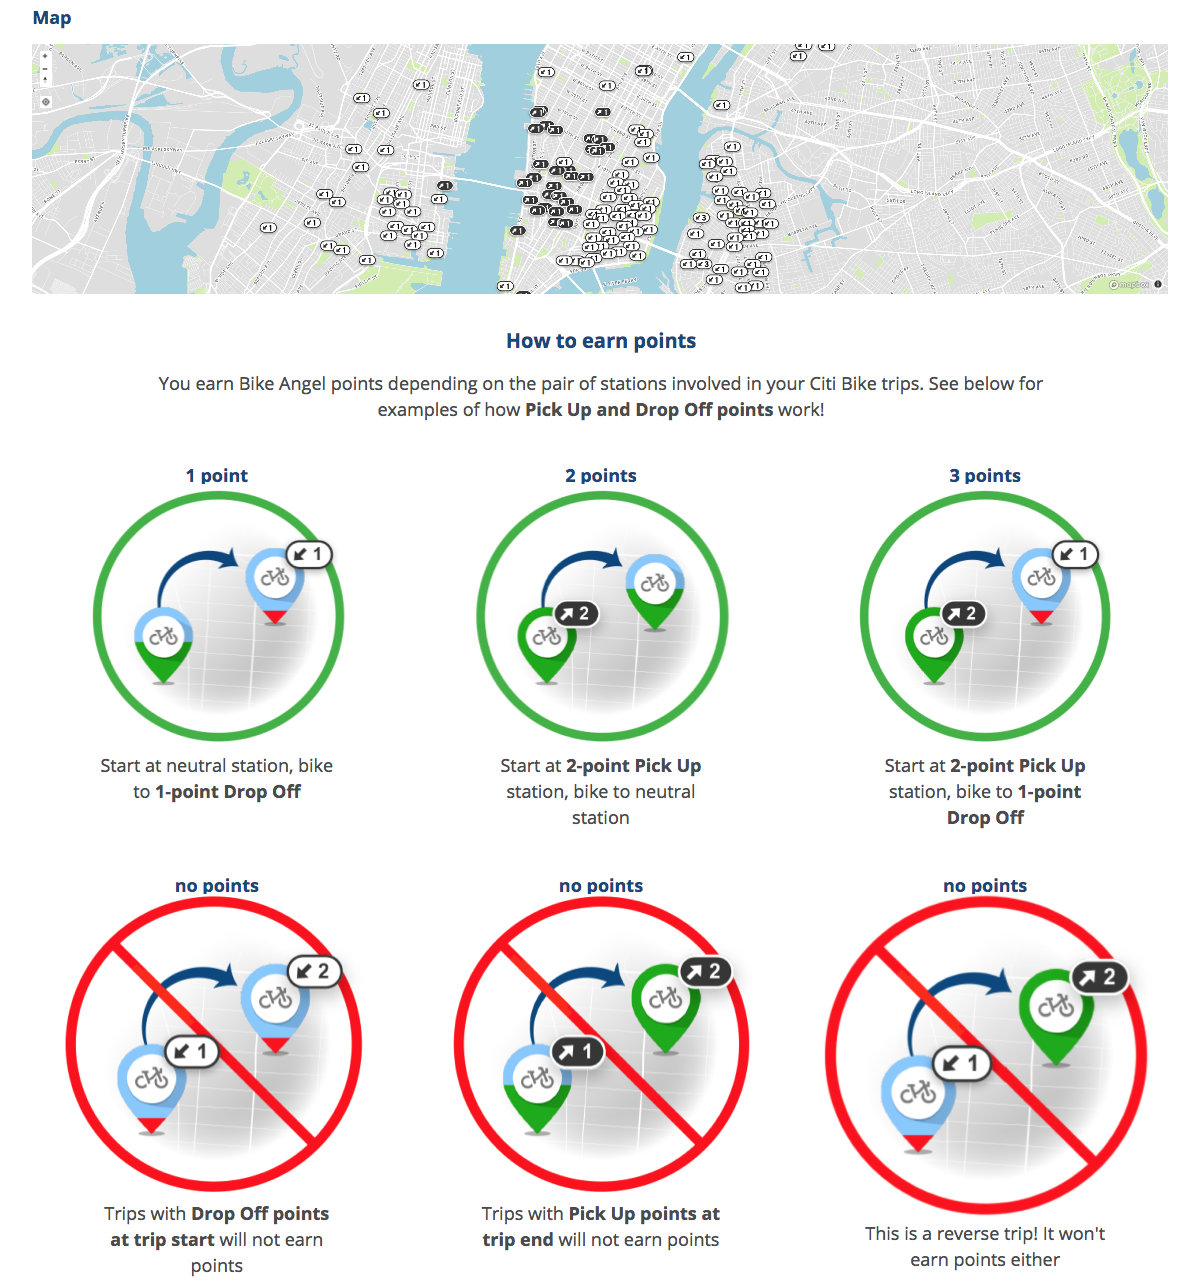
\includegraphics[width=.49\textwidth]{../Plots/screenshot_angels.png}
%\caption{Screenshot of Bike Angels website, displaying the dynamic map and explaining how to earn points.}
%\label{fig:screenshot_angels}
%\end{figure}
 %our work has had on the design of the Bike Angel program.

%Motivation is to understand when/how/where to use incentives to induce positive behavior

%Apply the standard BSS inventory model to Citi Bike's incentive scheme data

%Estimate the impact on out-of-stock events of each rental/return for which points where awarded

%Design different policies, distinguish between levels of static/dynamic

%Report on the influence on design in NYC

%\subsection{Related Work}

%Bike-sharing systems have become ubiquitous in American cities. Most of these systems are station-based, that is, they consist of a number of capacitated stations at which bikes can be rented or returned. The major operational challenge these systems face  is due to asymmetry in demand: stations in residential areas run out of bikes in the morning hours whereas the stations become full and then cannot have additional bikes returned.

%In this work, we investigate the impact of Citi Bike's incentive scheme. Referred to as \emph{Bike Angel} program, the incentive scheme was installed with our guidance in October 2015. A key feature of the incentive scheme, as suggested by \cite{OMahony2015}, is the categorization stations into ones at which rentals/returns are incentivized. Noticeably, labeling a station as a return station when such a station indeed has too few empty docks available can yield to outcomes in which the operator rewards, through the incentives,returns/rentals that have negative impact on the balance of the system.

%\subsection{Contribution} We apply a well-studied inventory model of bike-sharing stations to the problem of determining when to incentivize returns/rentals at stations. To do so, we compare the performance of various static and dynamic policies with respect to the estimated impact of incentivized trips on out-of-stock events. Additionally, we use predictive methods to estimate the probability of an incentivized trip occurring due to or independently of the incentives given. Thus, for a given cost parameter associated to each incentive point awarded, we find optimal subset of trips to incentivize.

%In order to accommodate practical constraints, we also investigate various different policies that are less dynamic in that decisions are made offline rather than on a minutely basis. We demonstrate the trade-offs between solution quality and online decision-making on Citi Bike's data-set, whilst also proving that in particular fluid sense, the optimal solution has a great deal of structure. Finally, we define a formal notion




\section{Data Analysis and Definitions}\label{sec:angel_data}

In this section, we describe the data-sets at our disposal, the system parameters we derive from them, and the models by which we evaluate the different policies for the incentive scheme.

\subsection{Data-Sets}

Our analysis relies on three different data-sets. First, we have a list of all trips in the system with origin location, destination location, and respective times of the start and the end of the trip \cite{citibikedata}. Second, we have a list that indicates which of the above trips were rewarded with points by the existing offline incentive policy (as well as whether the point was awarded for the rental, the return, or both) \cite{citibikeInternal}. Last, for each minute and each station in the system, we have the number of bikes reported to be at the station at that time as well as the total number of docks available \cite{citibikejson}.

We use data collected over three different time periods in 2016 in our analysis: 04/01--05/13 (base), 10/03--10/30 (training) and 10/31--12/14 (testing). The base period includes the most recent 6-weeks of data when no incentive program was in use, and represents the system before incentives were introduced. The training period involves the first 20 days of the winter data after incentives were introduced, and the remainder is used as the testing period. The base and training periods are used to help calculate the system parameters, such as the rental/return rates and the stochastic interpretation of the incentives' effect explained later in this section, and also serve as the training period for some of our incentive policy algorithms. The testing period is used to evaluate and compare our suite of policies. 

%Newly added.
%During the time periods from which our data is drawn, two 6-hour time intervals were incentivized in the Citi Bike system: 6AM-12PM and 4PM-10PM - we refer to them as the AM and PM periods respectively. All incentivized trip data comes from these two 6-hour time intervals. The daily total number of incentivized rentals/returns in the AM/PM for the test period are shown in Figure [?], where we see a generally equal distribution of rental/returns in the PM period, but a return-skewed distribution in the AM period. 

%\begin{figure}
%\centering
%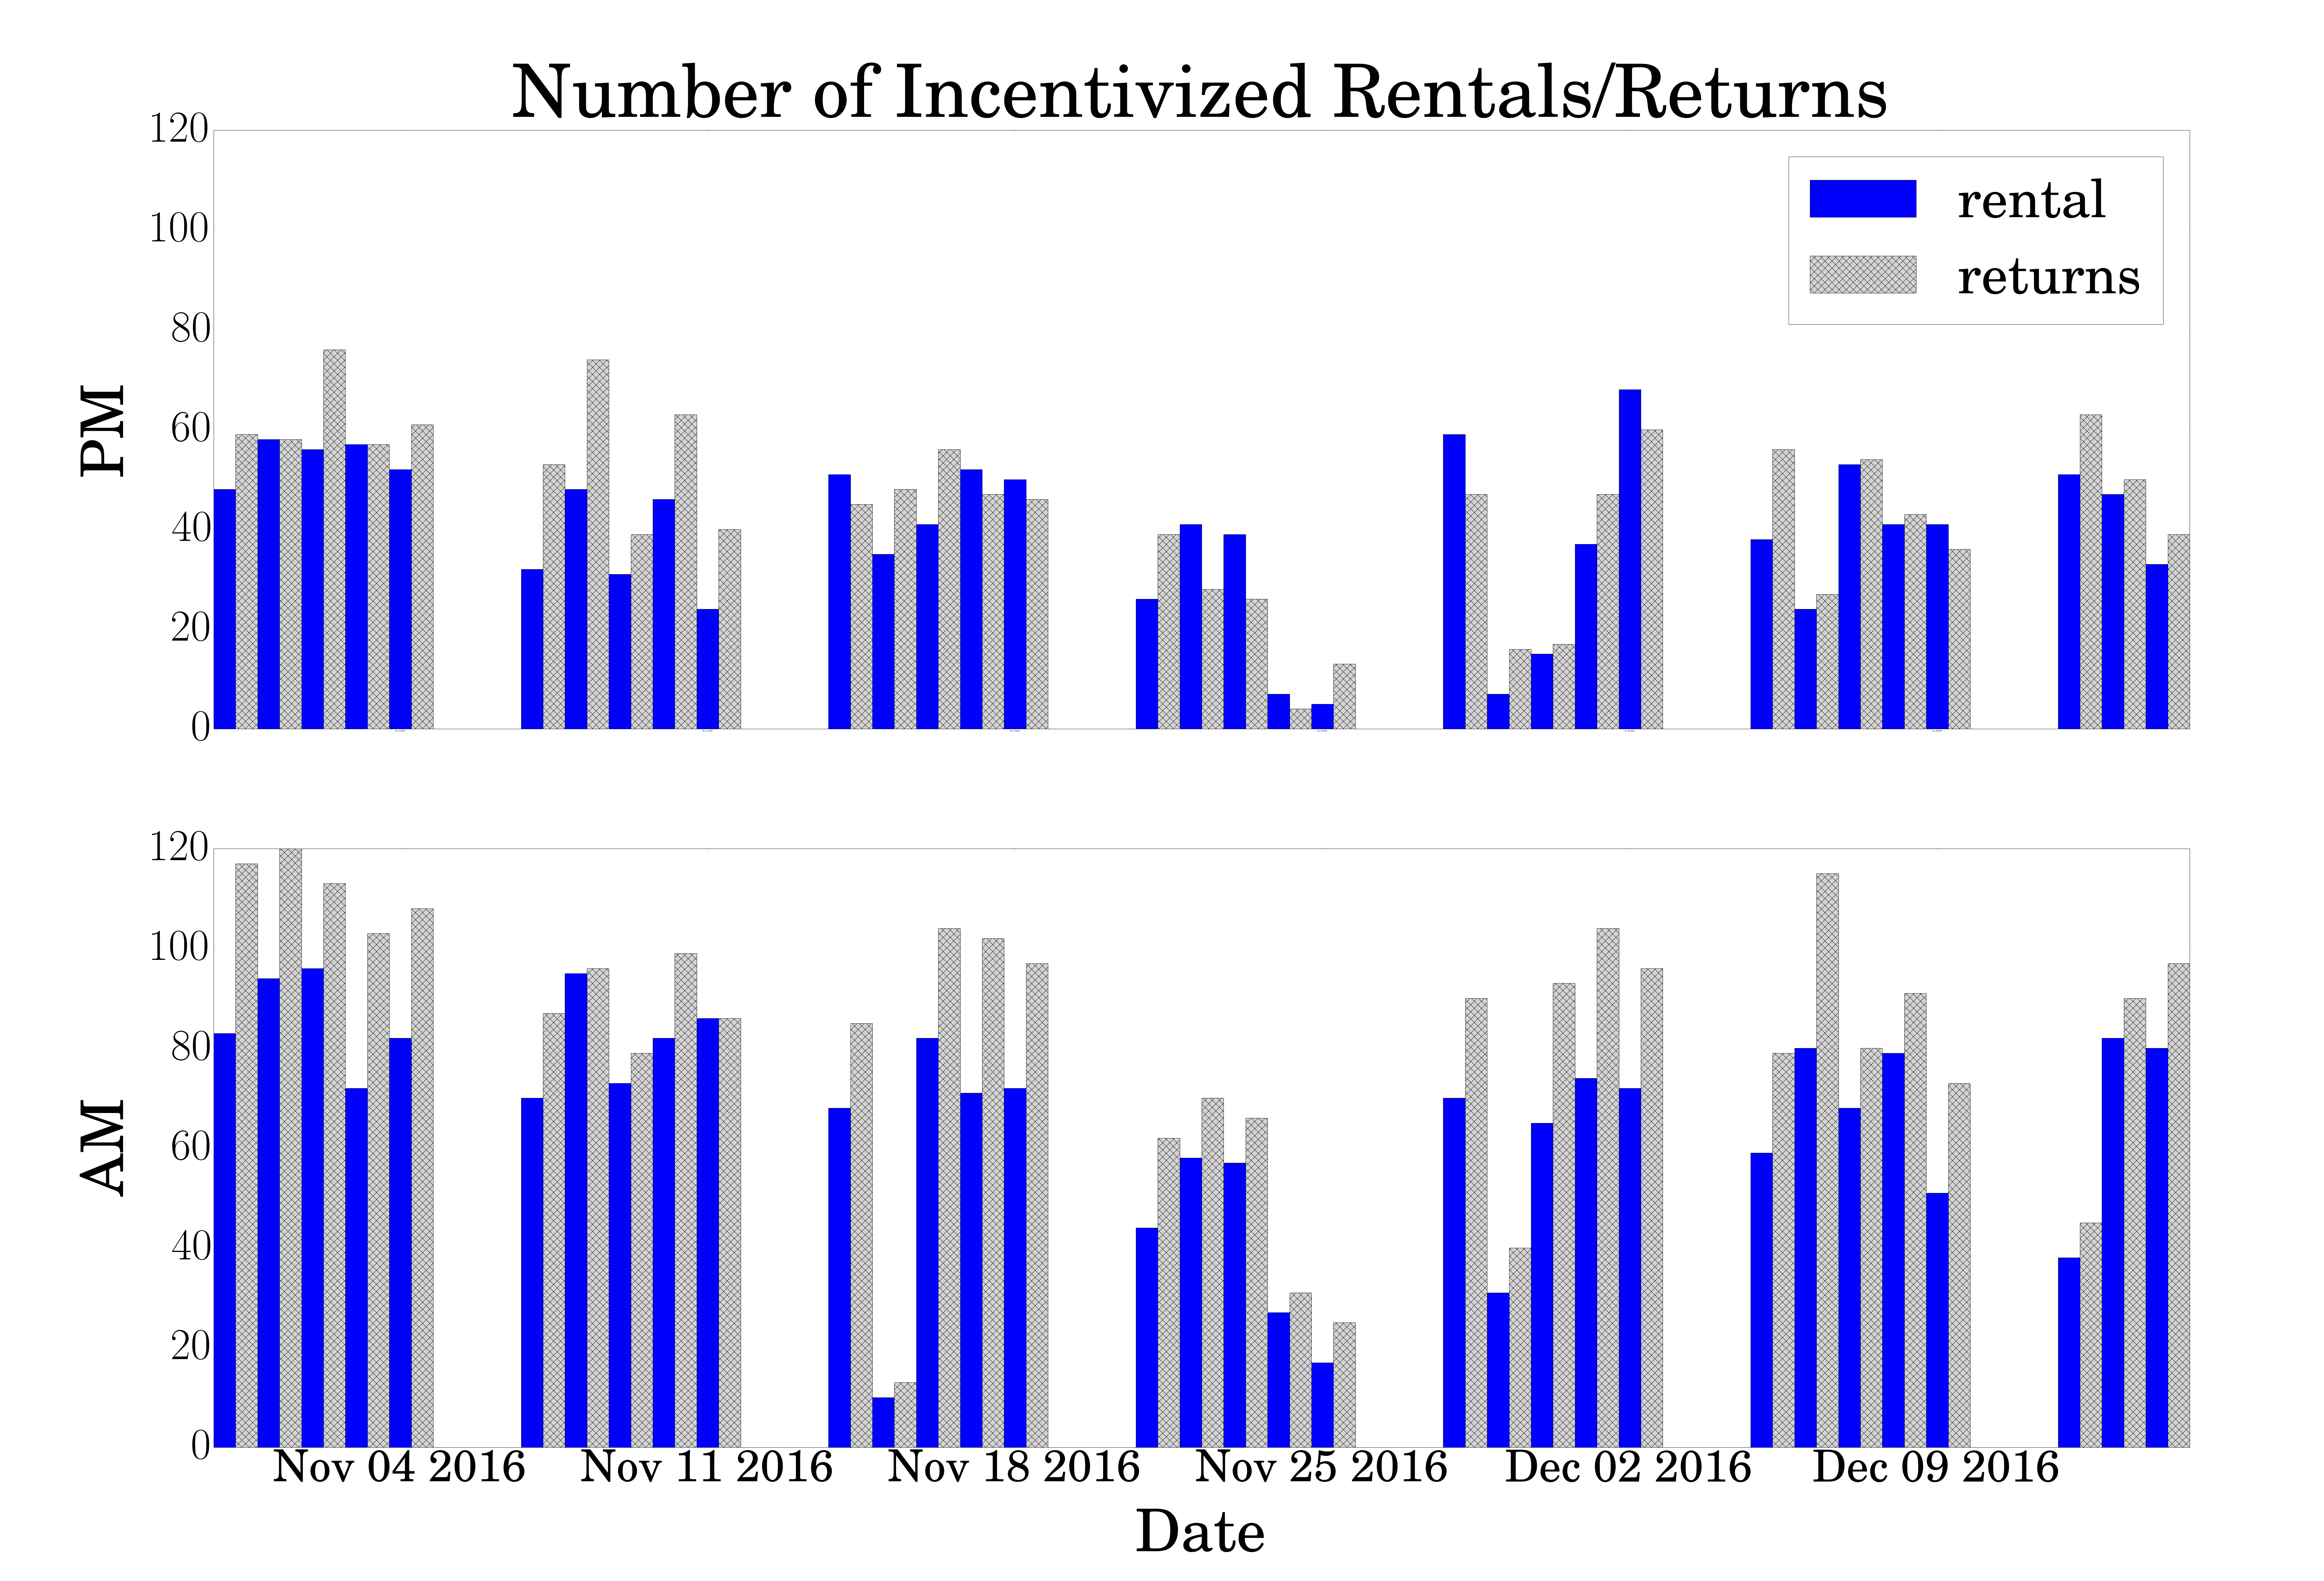
\includegraphics[width=.5\textwidth]{../SubmissionPlots/ActuallyUsed/Rental_Return.png}
%\caption{Total number of incentivized rentals/returns in the test period.}
%\label{fig:Incentivized Rentals/Returns}
%\end{figure}


\subsection{Data Censoring}

In our data, censoring proves to be a challenge as the data does not accurately reflect the true demand within the system. For example, a rider wanting to rent or return a bike to a station, with all docks empty or full respectively, cannot do so; thus, the corresponding demand would not be reflected in our data sets. To account for this problem of demand-censoring, when estimating average rental/return demand, we follow the methodology of \cite{o2015data} and examine station behavior on a minute-by-minute basis, only considering "active rental/return minutes", that is, minutes when a station has non-empty or non-full docks, respectively.

\subsection{Arrival and Departure Rates} 

Our analysis relies on three types of arrival and departure rates: regular-angel, incentive-angel, and non-angel rates. Regular-angel rates are the natural rental/return rates into a station for all angel riders combined, when no incentive is provided. The incentive-angel rates are the rates for the same set of customers when incentives are given. The non-angel rates are the rates for all other customers and are assumed to be unaffected by the incentive program. In our calculation of rates, we follow the work by \cite{o2015data} in assuming that the rates are independent across stations and calculate rates for every half-hour interval of the day starting from 12AM in the units bikes per minute.

To calculate the incentive-angel and non-angel rates, we take the data for a station's previous $q$ weekdays, and divide the total number of all arrival/departure trips by the specified riders by the total "active rental/return minutes" for each half-hour interval. In the results we present, $q$ is set to 20.

Formally, for each day $d$, station $s$, and time index $t$, let ($m_{d, s, t}^-$, $m_{d, s, t}^+$)  denote the active rental/return minutes, ($r_{d,s,t}^{a, +}$,$r_{d,s,t}^{a, -}$), ($r_{d,s,t}^{n, +}$, $r_{d,s,t}^{n, -}$) the number of arrival/departure trips for angel and non-angel riders respectively, and $D(d)$ be the set of the preceding $q$ weekdays before day $d$. Then the incentive-angel arrival rates $\lambda_{d, s, t}^{i, +}$ for day $d$, station $s$ and time index $t$, where $t \in \{0, 1, 2, ..., 47\}$ for the 48 half-hour intervals of the day (e.g. t=12 is 6 a.m.) are calculated as the rate per minute normalized to account for only active minutes, as follows (similar for departure rates $\lambda_{d, s, t}^{i, -}$ and non-angel arrival/departure rates $\lambda_{d, s, t}^{n, +}$ and $\lambda_{d, s, t}^{n, -}$):
\begin{equation}
\lambda_{d, s, t}^{i, +} =   \frac{\sum_{d' \in D(d)} r_{d',s,t}^{a, +}}{\sum_{d' \in D(d)} m_{d',s,t}^+} 
\end{equation}

%we define ($\lambda_{d, s, t}^{i, +}$, $\lambda_{d, s, t}^{i, -}$), ($\lambda_{d, s, t}^{n, +}$, $\lambda_{d, s, t}^{n, -}$) and ($\lambda_{d, s, t}^{r, +}$, $\lambda_{d, s, t}^{r, -}$) to be the pairs of incentive-angel, non-angel and regular-angel rental/return rates respectively for day $d$, station $s$ and time index $t$, where $t \in \{0, 1, 2, ..., 47\}$ for the 48 half-hour intervals of the day (e.g. t=12 is 6 a.m.). Further,


To estimate the regular-angel rates we used data from the base period, when no incentive program was offered. The regular-angel rates are assumed to be identical across days, and are calculated by dividing the angel rider's total number of all arrival/departure trips by the total "active minutes" in the base period for each half-hour interval, and applying a correction factor. The correction factor, $U$,  accounts for any general macro-change in system usage from the base time period to our testing time period. The correction factor is calculated by dividing the average daily total number of trips by non-angel riders during the training period by their average daily total number of trips during the  base time period. Finally, because the correction factor is an estimate of the change, we capped the regular-angel rates to be at most the incentive-angel rates to reflect our prior beliefs that incentivization actually helps our system. If we define $D$ to be the set of weekdays in the base time period and $U$ to be the correction factor, the regular-angel arrival rates are calculated as follows (similarly for departure rates):
\begin{equation}
\lambda_{d, s, t}^{r, +} = min(U \cdot  \frac{ \sum_{d' \in D} r_{d',s,t}^{a, +}}{ \sum_{d' \in D} m_{d',s,t}^+} , \lambda_{d,s,t}^{i, +} ) 
\end{equation}

\subsection{Stochastic View of Incentives}
Our analysis also relies on the probability that an incentivized rental/return would not have occurred if it had not been for the incentive; in particular, the rebalancing due to a rental/return that happens regardless of the incentives should not be attributed to the incentive scheme. We compute these probabilities for each day, station and half-hour interval by % and represents the probability that an incentive trip in this time-interval occurred due to the incentive. 
%To calculate them, 
dividing the difference of the incentive-angel and regular-angel rates by the incentive-angel rate. Formally, with $p_{d, s, t}^+$ and $p_{d, s, t}^-$ denoting the probabilities that a rental/return was triggered by the incentives, we compute these probabilities as %  and departure trip respectively, the probabilities of a rental/return occurring due to the incentives are calculated as follows (similarly for departure):
\begin{equation}
 p^+_{d, s, t} =  \frac{\lambda_{d, s, t}^{i, +} - \lambda_{d, s, t}^{r, +} }{\lambda_{d, s, t}^{i, +}}
 \end{equation}

\subsection{User Dissatisfaction Function}\label{ssec:udf}
The user dissatisfaction functions defined by \cite{raviv2013optimal} map the number of bikes at a station at a given time to the expected number of out-of-stock events over the course of a subsequent finite time-horizon. Formally, the functions assume that two exogeneous stochastic processes create arrivals of customers intending to return and rent bikes at the station. In our implementation, the stochastic processes are given by time-varying Poisson processes with rates being the non-angel rates. Crucially, the processes are assumed to be independent of the initial condition, that is, of the number of bikes at the station at the beginning of the time horizon. Then, each intended rental decreases the number of bikes in the station by 1 if a bike is available, i.e., if the number of bikes is at least 1. Intended returns increase the number of bikes by 1 if an empty dock is available at the station, i.e., if the number of bikes is less than the capacity of the station.  

Customers experience out-of-stock events if they intend a rental and the station is empty or if they intend a return and the station is full. Given the non-angel rental and return rates, one can then compute for a given station $s$ with $\ell$ bikes at time-index $t$, the expected number of out-of-stock events over a time-horizon beginning at time-index $t$, i.e., the expected number of intended returns  when the station is at capacity plus the expected number of intended rentals when the station is empty. We denote this expectation by $\phi_{s, t} (\ell)$.

%EXPLAIN HOW THE UDF USES DATA TO BE COMPUTED (NO DETAILS).

%In order to 

\begin{figure}
\centering
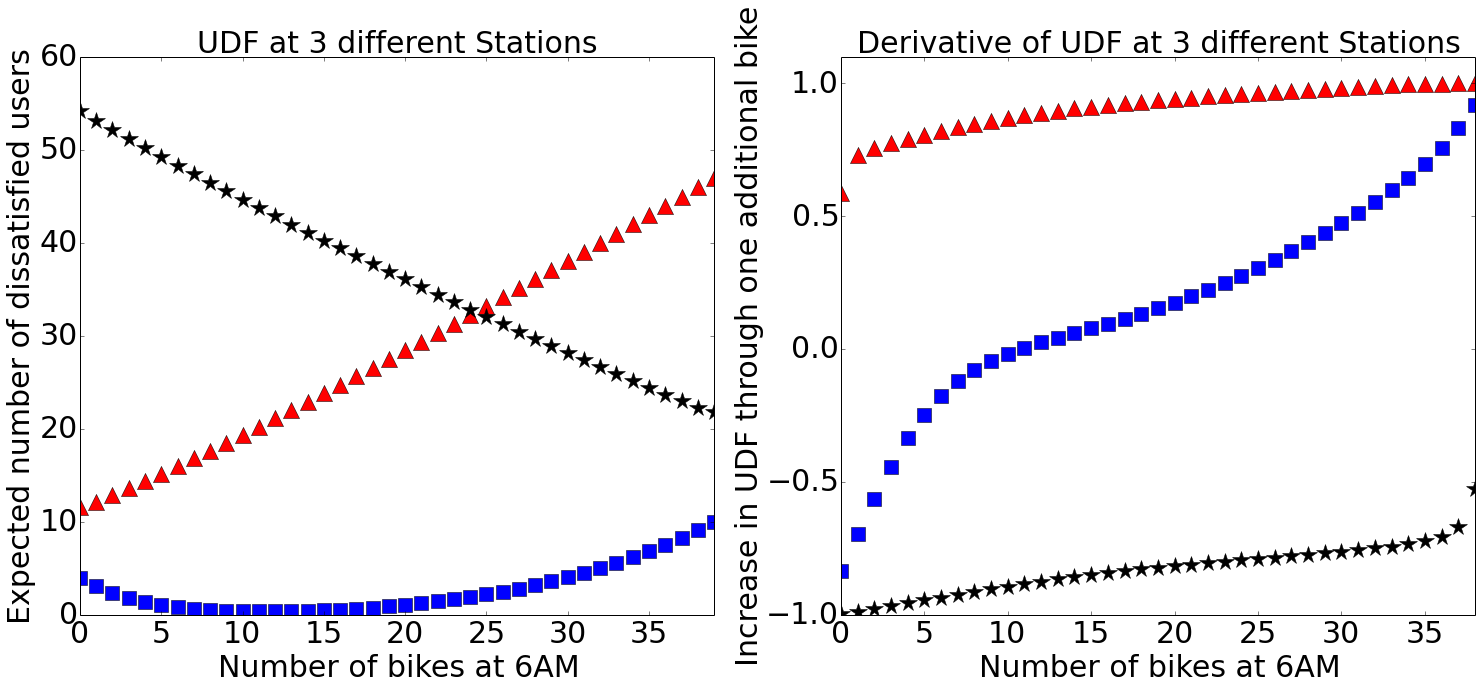
\includegraphics[width=.5\textwidth]{../Plots/UDFandDerivative2.png}
\caption{User dissatisfaction function $\phi_{s,t}(\cdot)$ and its discrete derivative for 3 different stations $s$ with the same capacity.}
\label{fig:UDFandDerivative}
\end{figure}

%Formally define the model as defined by \cite{raviv2013optimal}, describe the partition into half-hour intervals, emphasize that there's no point in taking smaller intervals, describe

\subsection{Performance Metrics and Policies}

For each incentivized return, we can estimate the reduction in out-of-stock events by computing the discrete derivative of the user dissatisfaction function with respect to one additional bike, evaluated  as a function of the number of bikes present in the station before the arrival. Similarly, for incentivized rentals, the estimated reduction in out-of-stock events equals the difference in the value of the user dissatisfaction function evaluated with one bike less and the actual number of bikes in the station.  In Figure \ref{fig:UDFandDerivative}, we display the respective user dissatisfaction functions and the value of the derivatives for three different stations at 6AM. Evaluating the user dissatisfaction functions for every half-hour interval, we estimate the impact of each rental/return on future out-of-stock events by evaluating the derivative of the user dissatisfaction function for that time-interval at the number of bikes present at the time of the return (and similarly for rentals). If we let $\delta_r$ denote the estimated reduction on future out-of-stock events for trip $r$,  let $\ell$ denote the bike-level at the station before the trip completed, and let $s$ and $t$ denote the station and time-index associated with the trip, we find that we may compute $\delta_r$ for a return as follows (similarly for rentals):

\begin{equation}
\delta_r = \phi_{s, t} (\ell) - \phi_{s, t} (\ell + 1)
\end{equation}

%The overall performance metric for a policy is defined to be the expected total reduction in out-of-stock events less the costs for any incentives given.  With the user dissatisfaction functions, we can estimate the impact of a single incentivized trip. More specifically, f

Though $\delta_r$ captures the impact of a return (rental) on the estimated number of out-of-stock events, it lacks two important aspects for our analysis. First, it lacks the cost associated with the incentive itself. To capture the operator's cost of the incentive scheme in the form of electronic gift cards, membership extensions, and other rewards (cf. \cite{bikeangels}), we include a constant cost parameter $\beta$ for every point awarded by an incentive scheme. Second, for every incentivized rental (return), we can incorporate the probability $p_{d,s,t}$ that the rental (return) would not have occurred without an incentive given; here, $d, s, t$ is the date, station and time index respectively in which the rental (return) occurred. This gives a stochastic perspective of the causal effects of incentives, in contrast to the deterministic assumption that incentivized rentals (returns) are always caused by the incentive. Using the above, we can define for every single incentivized return (rental) the performance of incentivizing it with both the deterministic and the stochastic perspective as % we can define the performance of incentivizing it by either viewing 

%In order to include the %As we consider the expected impact of a trip, it is worthwhile to not only include the impact of each incentivized trip on the user dissatisfaction functions, but also the 
%likelihoods that trips would have occurred without the incentives, we use the NEED A NAME FOR THESE IN STOCHASTIC VIEW OF INCENTIVES to define a stochastic and deterministic performance metric for a single trip. The deterministic evaluation assumes all incentivized trips occur due to  the incentive scheme only, and the expected reduction in out-of-stock events equals $\delta_{r}$ itself. The stochastic evaluation takes into account the probability of the trip occurring due to the incentive, and calculates the expected reduction to be $\delta_{r} * p_{d,s,t}$, where $d, s, t$ is the date, station and time index respectively in which the trip occurred. 

%Furthermore, when evaluating the performance metric for a policy we not only want to consider the expected impacts of the incentivized trips, but also account for the cost of giving incentives. Thus, we associate a fixed cost $\beta$ per awarded incentive point. This corresponds to the operator's cost of monthly rewards in the form of electronic gift cards, membership extensions, etc. \cite{bikeangels}.

%Let us define $\Delta_{r}$ to be the expected reduction on future out-of-stock events minus the cost of incentivizing for trip $r$. The deterministic and stochastic evaluation of $\Delta_r$ is calculated as follows:
\begin{equation}
    \Delta_r=
    \begin{cases}
       \delta_{r} - \beta & \text{ if deterministic}\\
       \delta_{r} \cdot p_{d,s,t}  - \beta & \text{ if stochastic}
    \end{cases}
\end{equation} 

Given $\Delta_r$ as a performance measure for incentivizing a single return (rental) $r$, we define the performance of a policy as the sum of all $\Delta_r$ corresponding to incentivized rentals (returns) $r$. Formally, denoting by $\tau$ the set of all rentals (returns) in the testing period, we define a policy $P$ as a function $P:\tau\to \{0,1\}$ identifying for each rental (return) $r$ whether or not $P$ incentivizes it. Then,   %   let us define a policy to be a mapping from the set of incentivized trips to the binary decision variable indicating whether a trip is incentivized. Thus let us define $\tau$ to be set of possible incentive trips, and a policy $P$ to be the function $P: \tau \to 0/1$.
to compute the overall performance $H(P)$ of a policy $P$ we compute
\begin{equation}
 H (P) =  \sum_{r \in \tau} P(r) \cdot \Delta_r 
\end{equation}



%Explain the set up of the problem, data collection methods \\
%Explain the Cost Curve function and what it represents \\
% \\



\section{Policies}\label{sec:angel_policies}

In this section, we define a number of incentive policies and identify the fundamental differences between offline and online policies.  During the time periods from which our data is drawn, two 6-hour time periods were incentivized in the Citi Bike system: 6AM-12PM and 4PM-10PM -- we refer to them as the AM and PM periods, respectively.  Since all of the incentivized trip data comes from only these two periods (cf. Figure \ref{fig:Incentivized Rentals/Returns}), we test/apply our policies only for these periods. Furthermore, each policy treats the two time periods independently, and calculates an incentive scheme for each time period and station. From the figure, we see a generally equal distribution of rental/returns in the PM period, but a return-skewed distribution in the AM period. 

\begin{figure}
\centering
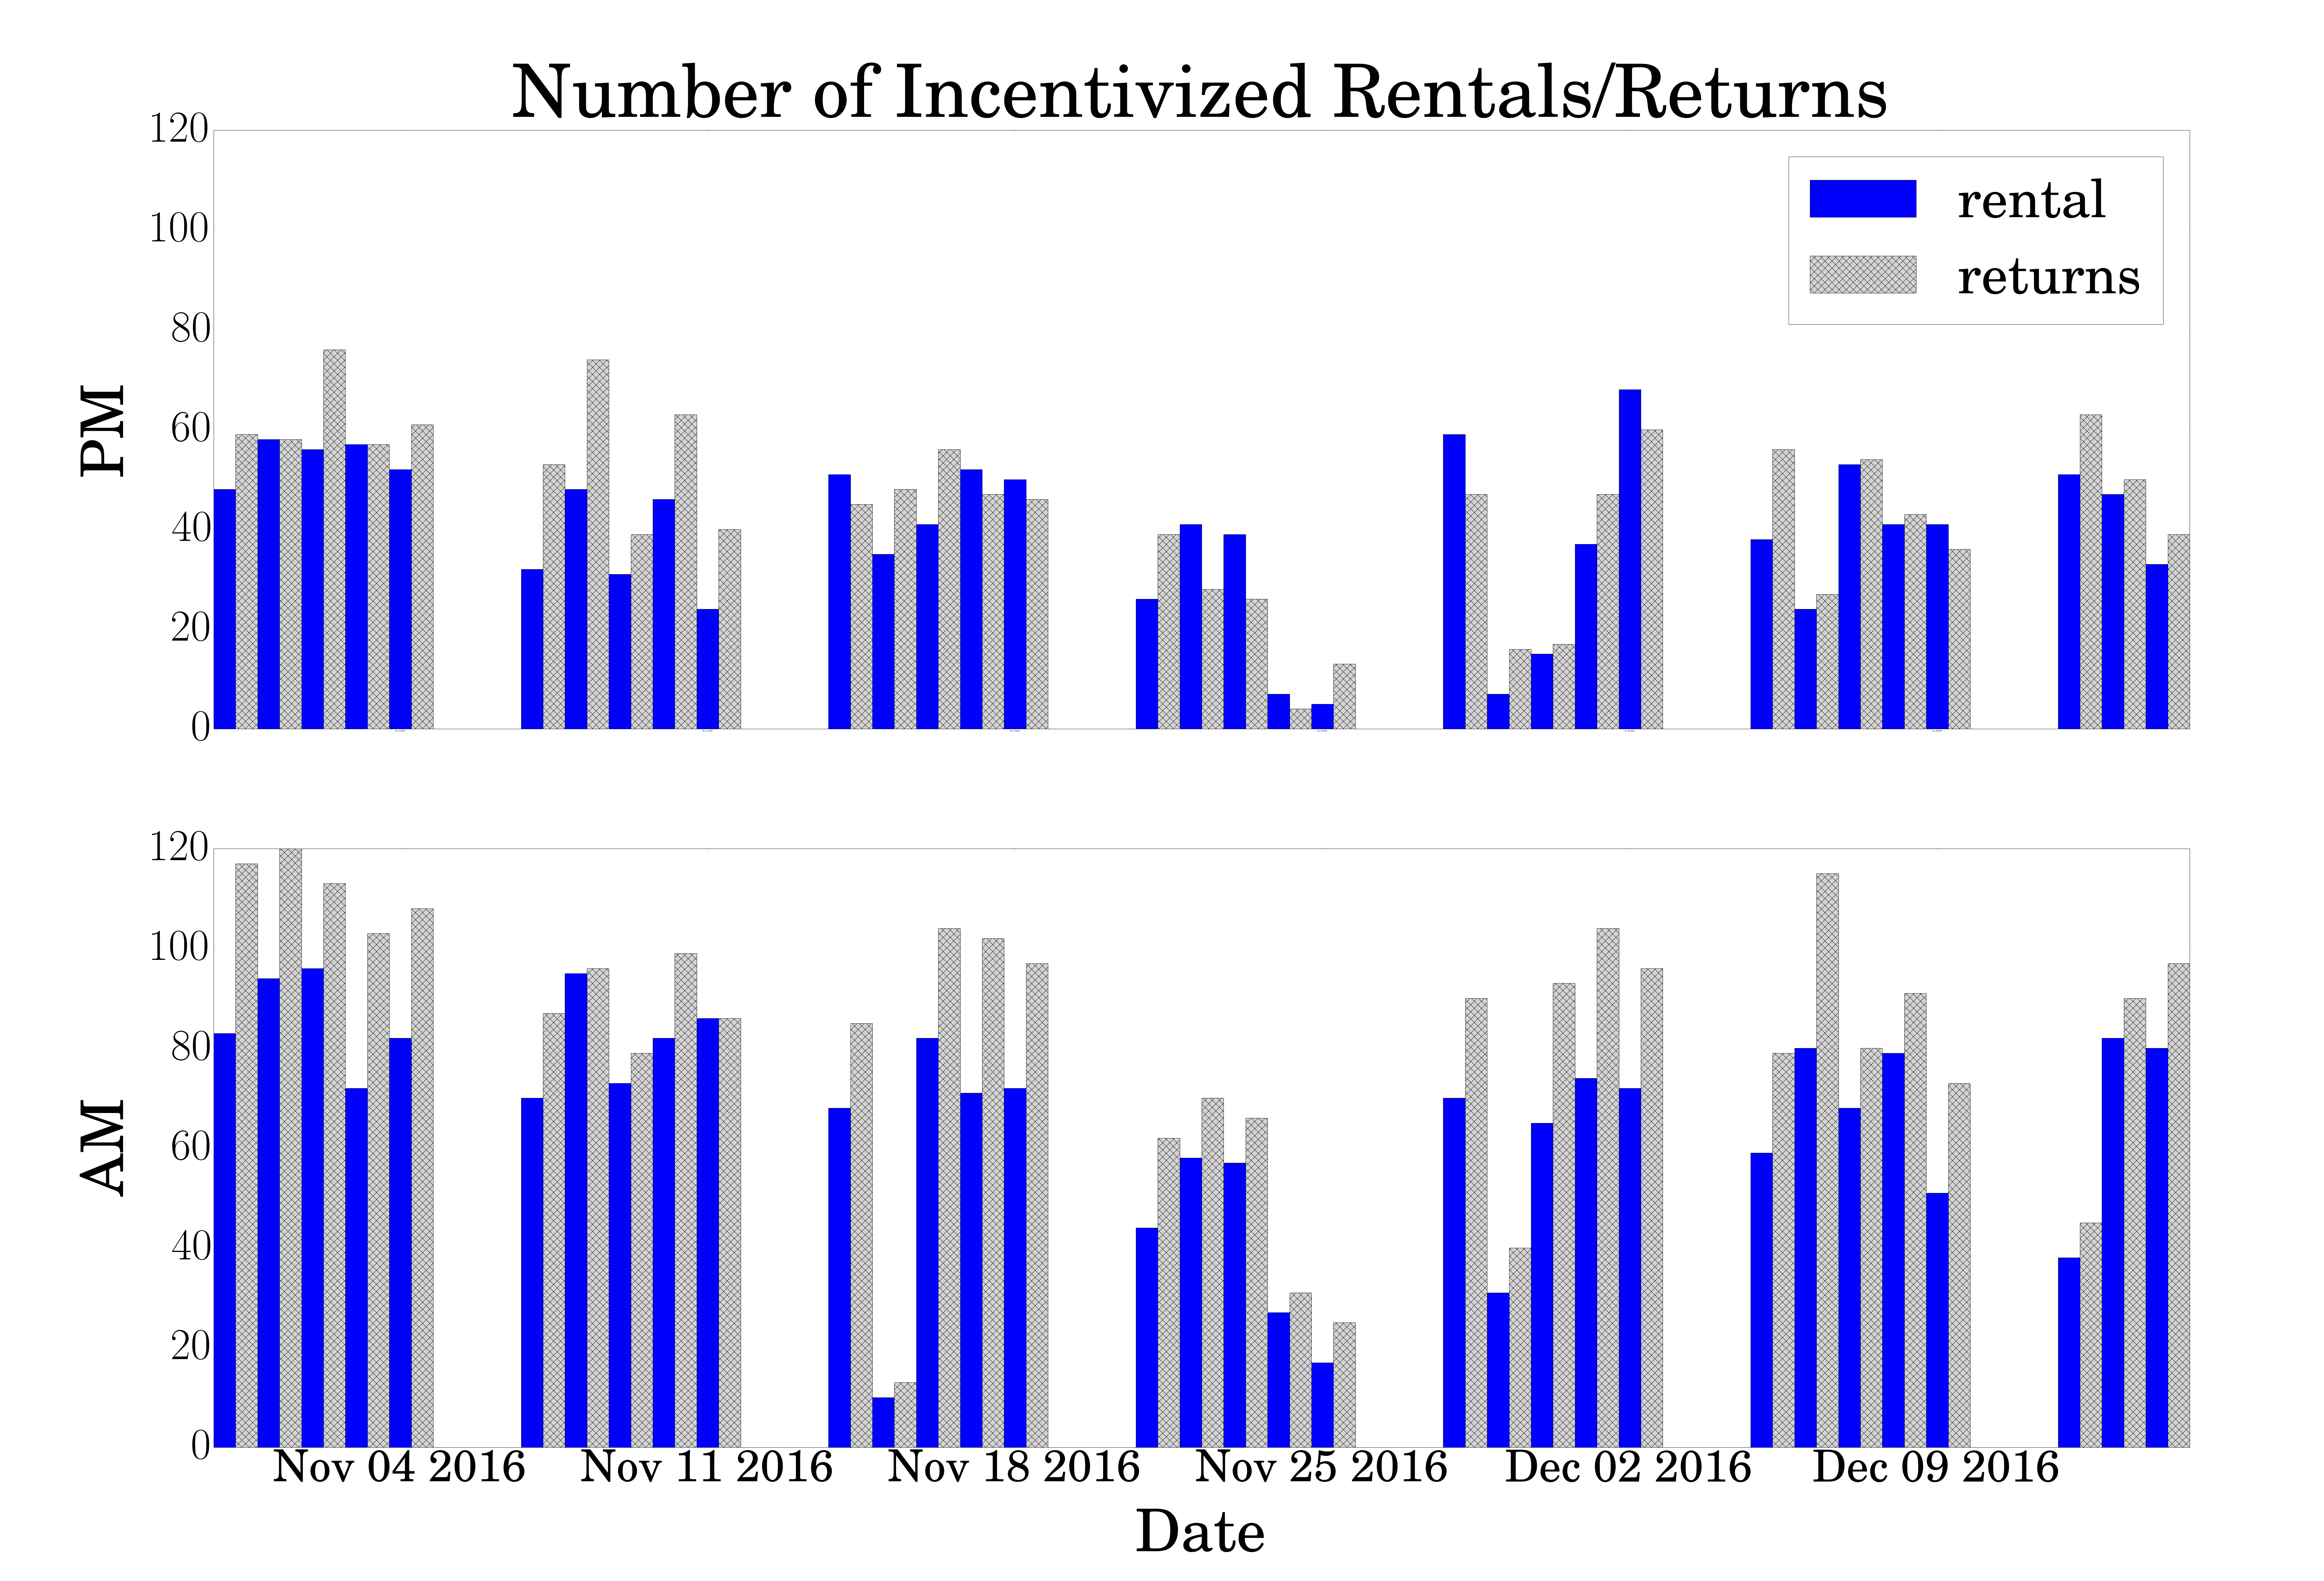
\includegraphics[width=.5\textwidth]{../SubmissionPlots/ActuallyUsed/Rental_Return.png}
\caption{Total number of incentivized rentals/returns in the test period.}
\label{fig:Incentivized Rentals/Returns}
\end{figure}

% While online policies thus h a downside with respect to The downside of such online decision making is the decreased perceived predictability of whether a (later) trip will be incentivized. The upside; however, is the increased efficiency of online policies as we will show in the next section. 	

\subsection{Offline Policies}

We first describe the offline policies. \emph{Offline} policies are characterized by the fact that the decision, for each AM/PM period, as to which interval will be incentivized for each station is made (irrevocably) at the beginning of that time interval (6AM and 4PM for AM and PM, respectively); in doing so, these policies have access to past data and the number of bikes at that time, i.e., 6AM and 4PM, respectively. %do not rely on 
(Note that this use of term offline is different from its use in other contexts, where offline often means that the algorithm has access to {\it all} of the data for the input to be optimized before needing to commit to any decision.) 

\subsubsection{Static}
The Static model is the simplest offline policy and was also the policy employed in Citi Bike at the time that this research project initiated. This policy determines a subset of stations to incentivize for which  the entire AM period is incentivized on every day, and similar subset is determined for the PM period. This model serves as a baseline against which all other policies are compared.

\subsubsection{Static Hindsight} 
The Static Hindsight model is an offline policy that chooses, for each station, the optimal continuous incentive period when looking back in hindsight for the past $q'$ weekdays. More precisely, the model assumes an incentive interval can start/stop every 30-minutes, starting from the beginning of the time period (e.g., 06:00 -- 07:30 or 07:00 -- 12:00 for the AM period), and chooses the incentive interval that achieves the highest performance when constrained on the past $q'$ weekdays of trip data. Throughout, we will use the term incentive interval to refer to such a continuous time period with these discrete start/end times. In our results, $q'$ is set to be 10. Thus, we let $D(d)$ denote the set of dates which are $q'$ days in hindsight;
we let $\tau(D(d), s)$ denote the possible morning incentive trips belonging to those dates and station $s$, and let $I_{d,s}$ to be the incentive interval for station $s$ on day $d$. Furthermore, let us say trip $r \in I$ if and only if the trip occurred during the interval $I$. The interval $I_{d,s}^\star$ chosen by Static Hindsight for the morning period is
\begin{equation}
\text{arg}\,\max\limits_{I}\ \sum_{r \in \tau(D(d), s)} \Delta_{r} \cdot 1_{r \in I} ,
\end{equation}
where the notation $1_{r \in I}$ means the indicator function that is equal to 1 if $r \in I$, and is 0, otherwise.

\subsubsection{Cluster Hindsight}
This offline policy uses a clustering of the stations to help make incentive decisions. As we describe in more detail below, the model first groups the stations by station dock-capacity, clusters each group by bike-level behavior, and finally chooses the optimal incentive interval for each cluster when looking back in hindsight (similar to Static Hindsight). 

We compute groups of stations by sorting them from smallest to largest capacity, and dividing them into $g$ roughly equal-size groups. %To be exact, we first group the stations into $g$ equal size groups, such that the smallest $\frac{1}{g}$ stations form the first group. 
The intuition for the grouping is our prior belief that station activity level is highly correlated with station capacity size and it is unwise, for example, to compare stations with bike-capacity 5 with stations of bike-capacity 60. The actual data-points used to cluster are 12-dimensional vectors consisting of the 12 half-hour interval bike-level percentages (bike-level divided by station dock capacity) for a station and date. The data points were obtained from our training data period, and bike-level percentages, rather than absolute values, were used to normalize the data points. To cluster each group of stations, we run the k-means clustering algorithm (k-centroids) with the objective of minimizing the distortion, which is defined to be the sum of the squared Euclidean distances between each vector and its centroid. Finally, our model uses a hard labeling system to associate each station with a single cluster (since for each station we have multiple points corresponding to distinct dates), and labels a station as belonging to the cluster for which its data points are most prevalent. 

To calculate the actual incentive intervals for each cluster, the model finds the optimal single, continuous incentive interval when looking back in hindsight of $q'$ weekdays for the stations in the cluster. Then let us define $C(s)$ to be the cluster of stations which $s$ belongs to. The interval that the model chooses is as follows:
\begin{equation}
I_{d,s}^\star= \text{arg}\,\max\limits_{I}\ \sum_{s' \in C(s)} \sum_{r \in \tau(D(d), s')} \Delta_{r} \cdot 1_{r \in I}
\end{equation}

The number of groups and the number of clusters are hyper-parameters of the model. To fit these parameters and avoid high bias/variance problems, k-fold cross-validation was used with our training data, and the parameters with the best average scores were chosen. Due to the temporal aspect of the data (e.g., weather plays a big role in system behavior) the k-folds were also divided to maintain the temporal order. The final parameters used in our results are $g$ = 10, $k$ = 3 and $q'$ = 10.

\subsubsection{Fluid Model}

A natural way to use the incentive-angel and non-angel rates to define an offline policy is by defining a so-called fluid model, in which it is assumed that exactly the expected number of rentals and returns occurs continuously per unit of time. Within such a model, it is easy to find the interval during which incentivizing minimizes the (fluid) number of out-of-stock events. In fact, one can show that under mild assumptions on the data, it is guaranteed that incentivizing over a single interval is optimal in such a model.

Though fluid models have successfully been applied to operational questions in bike-sharing, e.g., in \cite{jianetal}, we found in our analysis that the fluid model was vastly dominated by all other models; thus, we omit both its formal definition here and its performance in the results section.

\subsection{Offline Benchmark}

Offline policies are constrained in two ways: first, by the fact that we allow them to incentivize only during subintervals, as opposed to incentivizing, say, from 6-8AM and then again from 9-10AM but not in between; second, since the decision is based solely on the number of bikes at each station at 6AM, they lack information about demand later in the course of the day. To distinguish between the lack of information and the constraint of incentivizing only during a subinterval, we define the following \emph{static optimal} benchmark that has access to full information, but is constrained to incentivize only during a subinterval.

\subsubsection{Static Optimal}
The static optimal model is not a feasible policy since it assumes future knowledge that is not given in practice; instead, it is a model built in hindsight to benchmark offline policies. More specifically, for each week, station and AM/PM period, the Static Optimal model considers in hindsight, with complete knowledge, the best possible single continuous incentive period in which to incentivize.

\subsection{Online Policies}

In contrast to the offline policies described above, online policies gain information over the course of the day and thus are able to adopt whether or not to incentivize at a given station at a given time. We define only a very simple set of online policies.

\subsubsection{Dynamic}
The Dynamic model is a completely online policy that chooses in real-time for each trip whether or not it is incentivized to guarantee perfect efficiency. Formally, the model incentivizes all trips with $\Delta_r>0$ (cf. Equation 5), i.e., the performance is exactly the sum of all trips that contribute positively to the objective. This policy serves as an upper-bound on what any policy can possibly achieve within our analysis. 

\subsubsection{Dynamic CC (X)}
Beyond the fully dynamic model, we define a parameterized family of policies, wherein each policy breaks up the incentive period into intervals and the parameter X dictates the size of the intervals. For a given X, Dynamic CC starts at the beginning of each AM/PM period and decides every X minutes whether or not to incentivize trips for the next X minutes. To decide whether to incentivize the next X minutes, the model simulates the occurrence of one incentivized trip with the current number of bikes and empty docks at the station. If the simulated value of $\Delta_r$ is positive, Dynamic CC chooses to incentivize trips at the station for the next X minutes. For example, the Dynamic CC 15 model at 6 AM will check the station's current number of available bikes and docks, and simulate an incentivized trip for that user dissatisfaction function and that number of bikes and docks available. If the $\Delta_r$ value for this trip is positive, it will choose to incentivize the station from 06:00--06:15. Then, at 06:15 it simulates a new trip, based on updated information, to determine whether or not to incentivize from 06:15--06:30. 

We consider the Dynamic~CC policy for $X\in\{15,30,60,120\}$. Furthermore, one could also view the Dynamic model as Dynamic CC with $X=0$.

%Formally, for station $s$ and day $d$, let $t_x$ be the X-minute interval in question, $I(t_x)$ to be the binary incentive decision to incentivize or not, and $t$ be the half-hour interval to which $t_x$ belongs. Further, let $l_{s,t_x}$ be the bike-level at time $t_x$ and $\phi_{s,t}(l)$ be defined as in equation (??). Then $I(t_x)$ for arrival-incentives are calculated as follows: DOESN"T SEEM VERY PLEASING TO THE EYE. HOW SHOULD WE CHANGE THIS?
%\begin{equation}
%    I(t_x) = 
%    \begin{cases}
%      1  \{ \phi_{s,t}(l_{s,t_x}) - \phi_{s,t} (l_{s,t_x} + 1) - \beta \ge 0 \} & \text{ if deterministic} \\
%      1  \{ (\phi_{s,t}(l_{s,t_x}) - \phi_{s,t} (l_{s,t_x} + 1)) * p_{d,s,t} - \beta \ge 0 \} & \text{ if stochastic} \\
%    \end{cases}
%\end{equation} 




%\subsection{Fluid}
%The Fluid model is an offline policy that uses an estimation of the bike-level throughout the day to choose an incentive period which minimizes out-of-stock events. Given a potential incentive period as well as the starting bike-level at a station for the time period, the model uses the arrival/departure rates defined previously (c.f. equation (??)) to estimate the bike-levels after every 30-minute interval. Furthermore, if the estimated bike-level after a 30-minute interval is either below zero or above the dock-capacity of the station, the absolute quantity below zero or above the capacity can estimate the out-of-stock events occurring during the 30-minute interval. Thus to find the total estimated count of out-of-stock events occurring during the morning/afternoon period, the Fluid model estimates the fluid bike-level after each 30-minute interval, adds the interval's out-stock-events to the total count, and if necessary caps the bike-level below by zero and above by the dock-capacity, before moving onto the next 30-minute interval. 
%
%When considering the total estimated out-of-stock events, it is worthwhile to not only consider the out-of-stock events occurring during the period, but also the estimated future out-of-stock events from the resulting bike-level at the end of the period. The model incorporates this into its calculation by evaluating the user-dissatisfaction function at the estimated finishing bike-level and adding this to the total count. To find the best incentive period, the Fluid model chooses the incentive period which minimizes the total estimated out-of-stock events.
%
%Formally, let us define $f_{d,s,t}$ to be the expected bike-level for station $s$, on day $d$ and 30-minute time interval $t \in \{0, 1, 2,...,47\}$. Also for a station let $d_s$ be the dock-capacity, and $I$ be the incentive period indicating which 30-minute time intervals to incentivize. If the station is an arrival incentivized station for the morning period, $f_{d,s,t}$ can be calculated recursively as follows (similarly for afternoon and departure incentives):
%\begin{equation}
%    f_{d,s,t}=
%    \begin{cases}
%      \text{actual bike-level at 6 a.m.}, & t=12 \\
%      min(max(f_{d,s,t-1}, 0), d_s) + 30( \lambda_{d,s,t}^{r, +} +  \mu), & t \not\in I\\
%      min(max(f_{d,s,t-1}, 0), d_s) + 30(\lambda_{d,s,t}^{i, +} + \mu), & t \in I\\
%    \end{cases}
%\end{equation} 
%where
%\begin{equation}
%\mu =  - \lambda_{d,s,t}^{r, -} + \lambda_{d,s,t}^{n, +} - \lambda_{d,s,t}^{n, -}
%\end{equation}
%Finally, using the user-dissatisfaction function $\phi_{s,t} (l)$, the Fluid model chooses its optimal incentive period $I^*$ as such for the morning period (similarly for the afternoon):
%\begin{equation}
%I^*= \text{arg}\,\min\limits_{I}\  \phi_{s,24} (l) + \sum_{t=13}^{24} (0 - f_{d,s,t})^+ + (f_{d,s,t} - d_s)^+
%\end{equation}
%where
%\begin{equation}
%l = min(max(f_{d,s,24}, 0), d_s)
%\end{equation}



%
%
%\subsection{Offline/Online Decision Making}
%The different policies we analyze can be divided into two fundamental groups: offline and online policies. The offline policies choose, prior to the start of each morning/afternoon period,  a single continuous time period for which the station is incentivized. The motivation for a single continuous incentive interval is given by Proposition 1 and the performance of the Static Optimal, a static policy with perfect hindsight, shown later. Online policies, on the other hand, make dynamic decisions throughout the morning/afternoon periods and are not restricted to one continuous incentive interval. As we will see in the results section, that flexibility, combined with the additional information, makes the online policies more efficient. However, that improved efficiency comes at the cost of increased complexity and decreased perceived predictability for the user. 

\section{Results}\label{sec:angel_results}

In this section, we present the performance of a number of policies when run with varying cost-parameter for both the AM and PM periods.  %We then first identify key take-aways from the results, and later provide analysis on these observations. 
The data-set for the test period, on which our analysis relies, consists of a total of 4944 trips in the AM and 2800 trips in the PM, across 147 stations. We focus our analysis on the deterministic regime in which we assume that an incentivized rental/return is always triggered by the incentive given and would not have occurred otherwise. Thereafter, we contrast those results with the ones in the stochastic regime. The scores for the former are displayed in Table \ref{table:det} and for the latter in Table \ref{table:stoch}. All scores are given as the fraction of improvement of the % evaluation and later provide analysis on the stochastic evaluation results. The deterministic performance scores for both the morning (AM) and afternoon (PM) are presented in Table [1], and the scores are relative scores compared to the perfectly 
optimal dynamic policy (i.e., each policy's absolute score is divided by the dynamic policy's absolute score). We begin by giving a high-level summary of our most interesting findings before providing more details for each of them.

%In this section, we present and analyze both the deterministic and stochastic performance results of the different policies when run with various cost parameters. The overall analysis is performed on a total of 147 incentive stations during the test period, which accounts to a total of 4944 AM trips and 2800 PM trips. In the next subsections, we will first identify key take-aways from the deterministic results, and provide analysis on these observations. Afterwards, we will examine the stochastic results and what they indicate. The deterministic and stochastic performance results are presented in Table 1 and 2 respectively. All scores presented in both tables are relative scores compared to the optimal dynamic policy (i.e. each policy's absolute score divided by the dynamic policy's absolute score). 

\begin{table}
\caption{Policy Performance Scores in Deterministic Regime.}
\label{table:det}
\begin{tabular}{ |l| l| *5{c|}  }
\hline
\multirow{2}{*}{Time} & \multirow{2}{*}{Policies} & \multicolumn{5}{ c| }{Cost Parameter}\\  \cline{3-7}
& & 0.0 & 0.1 & 0.2 & 0.3 & 0.4 \\ \hline
\multirow{9}{*}{AM} & Dynamic & 1.0 & 1.0 & 1.0 & 1.0 & 1.0 \\
 & Stat. Opt. & 0.985  & 0.981& 0.976 & 0.97 & 0.961  \\
 & Static & 0.939  & 0.911 & 0.870 & 0.809 & 0.715 \\
 & Stat. HS & 0.960 & 0.947 & 0.929 & 0.905 & 0.873 \\ 
 & Clus. HS & 0.961 & 0.944 & 0.918 & 0.887 & 0.845 \\ 
 & Dyn 15 & 1.0 & 1.0 & 1.0 & 1.0 & 1.0\\ 
 & Dyn 30 & 0.995 & 0.994 & 0.993 & 0.992 & 0.990 \\ 
 & Dyn 60 & 0.989 & 0.984 & 0.980 & 0.977 & 0.969 \\ 
 & Dyn 120 & 0.967 & 0.953 & 0.944 & 0.940 & 0.924 \\
 \hline
\multirow{9}{*}{PM} & Dynamic & 1.0 & 1.0 & 1.0 & 1.0 & 1.0 \\
 & Stat. Opt. & 0.980 & 0.977 & 0.974 & 0.972 & 0.967\\
 & Static & 0.844 & 0.777 & 0.680 & 0.538 & 0.318 \\
 & Stat. HS & 0.943 & 0.934 & 0.917 & 0.891 & 0.858 \\ 
 & Clus. HS & 0.932 & 0.917 & 0.897 & 0.866 & 0.830 \\ 
 & Dyn 15 & 1.0 & 1.0 & 1.0 & 1.0 & 1.0 \\ 
 & Dyn 30 & 0.986 & 0.984 & 0.982 & 0.983 & 0.980 \\ 
 & Dyn 60 & 0.975 & 0.965 & 0.956 & 0.958 & 0.951 \\ 
 & Dyn 120 & 0.949 & 0.926 & 0.909 & 0.919 & 0.904 \\
 \hline
\end{tabular}
\caption*{Relative performances of each policy during AM and PM periods compared to the completely online policy under the deterministic performance evaluation.
}
\end{table}

\begin{table}
\caption{Policy Performance Scores in Probabilistic Regime.}
\label{table:stoch}
\begin{tabular}{ |l| l| *4{c|}  }
\hline
\multirow{2}{*}{Period} & \multirow{2}{*}{Policies} & \multicolumn{4}{ c| }{Cost Parameter}\\  \cline{3-6}
& & 0.0 & 0.01 & 0.1 & 0.2 \\ \hline
\multirow{9}{*}{AM} & Dynamic & 1.0 & 1.0 & 1.0 & 1.0  \\
 & Stat. Opt. & 0.979 & 0.973 & 0.945 & 0.912  \\
 & Static & 0.928 & 0.916 & 0.771 & 0.479 \\
 & Static HS & 0.957 & 0.944 & 0.878 & 0.796 \\ 
 & Clus. HS & 0.958 & 0.931 & 0.831 & 0.699 \\ 
 & Dyn 15 & 1.0 & 1.0 & 1.0 & 1.0\\ 
 & Dyn 30 & 0.995 & 0.995 & 0.993 & 0.991 \\ 
 & Dyn 60 & 0.985 & 0.870 & 0.832 & 0.773 \\ 
 & Dyn 120 & 0.966 & 0.68 & 0.612 & 0.514 \\
 \hline
\multirow{9}{*}{PM} & Dynamic & 1.0 & 1.0 & 1.0 & 1.0  \\
 & Stat. Opt. & 0.978 & 0.971 & 0.943 & 0.917  \\
 & Static & 0.923 & 0.903 & 0.646 & 0.15 \\
 & Stat. HS & 0.967 & 0.948 & 0.883 & 0.784 \\ 
 & Clus. HS & 0.958 & 0.935 & 0.839 & 0.682 \\ 
 & Dyn 15 & 1.0 & 1.0 & 1.0 & 1.0\\ 
 & Dyn 30 & 0.992 & 0.990 & 0.992 & 0.99 \\ 
 & Dyn 60 & 0.982 & 0.889 & 0.850 & 0.807 \\ 
 & Dyn 120 & 0.960 & 0.823 & 0.756 & 0.702 \\
 \hline
\end{tabular}
\caption*{Relative performance of each policy during AM and PM periods compared to the completely online policy under the probabilistic performance evaluation.}
\end{table}



\subsection{Key Observations of Deterministic Results}
Considering the rows indexed by Static for both AM and PM periods and both tables, it is noticeable that the static policy performs quite well, especially in the regime with low cost parameters, which is strong evidence of the operator's domain expertise in the initial choice of incentivized stations. Next, we observe the near-optimal performance of the Static Optimal benchmark across all cost parameters; this supports our decision to restrict the offline policies to  incentivize only over sub-intervals. For the dynamic policies, we observe a smooth decrease in performance as we transition from the maximally dynamic to more static policies, which highlights the trade-offs between efficiency and simplicity in the policies. Noticeably, none of the offline policies handle high cost-parameters well. Last, we observe a general decrease in performance from the AM to PM period, indicating that the system behavior is more erratic in the afternoon.
 
\subsubsection{Static Performance}
At first glance, the strong performance of the Static policy in Table \ref{table:det} (0.939 in the AM without costs) may seem surprising. It is explained, however, by the operator's domain expertise when deciding which stations to include in the incentive scheme. Its degrading performance with increased costs is explained by the fact that the policy does not adapt to the shrinking set of trips with positive impact as costs increase.
%In considering the Static policy's results in Table 1, it is interesting to note the policy's strong performance with no cost parameters, scoring up to 0.939 in the AM period. In hindsight, this is not surprising and exemplifies Citi Bike's domain expertise when setting the initial incentive policy. Likewise, the degrading performance with increased costs is unsurprising, since the policy does not adapt to the shrinking set of trips with positive impact as the cost increases. % shrink with higher costs.

Despite its reasonable performance in the AM in the regime without costs, the Static policy is still dominated by all policies across  all cost parameters. This is especially prominent in the PM period, where differences range from 9\% (Stat. HS)  up to 15\% (Dyn 15) even without cost parameters; the differences are even higher when accounting for costs. All of the incentivized trips in the PM, grouped by their improvement on the objective, $\delta_r$, are visualized in Figure \ref{fig:Static Performance}. Though the vast majority of incentivized trips have positive-impact, the other policies are able to accurately exclude those trips that do not, thus achieving higher performance.  These results exemplify the importance of a data-driven approach to improve the Bike Angels program. For example, even a rather simple policy with minimal overhead, such as Static Hindsight, significantly improves the efficiency of the incentives.

\begin{figure}
\centering
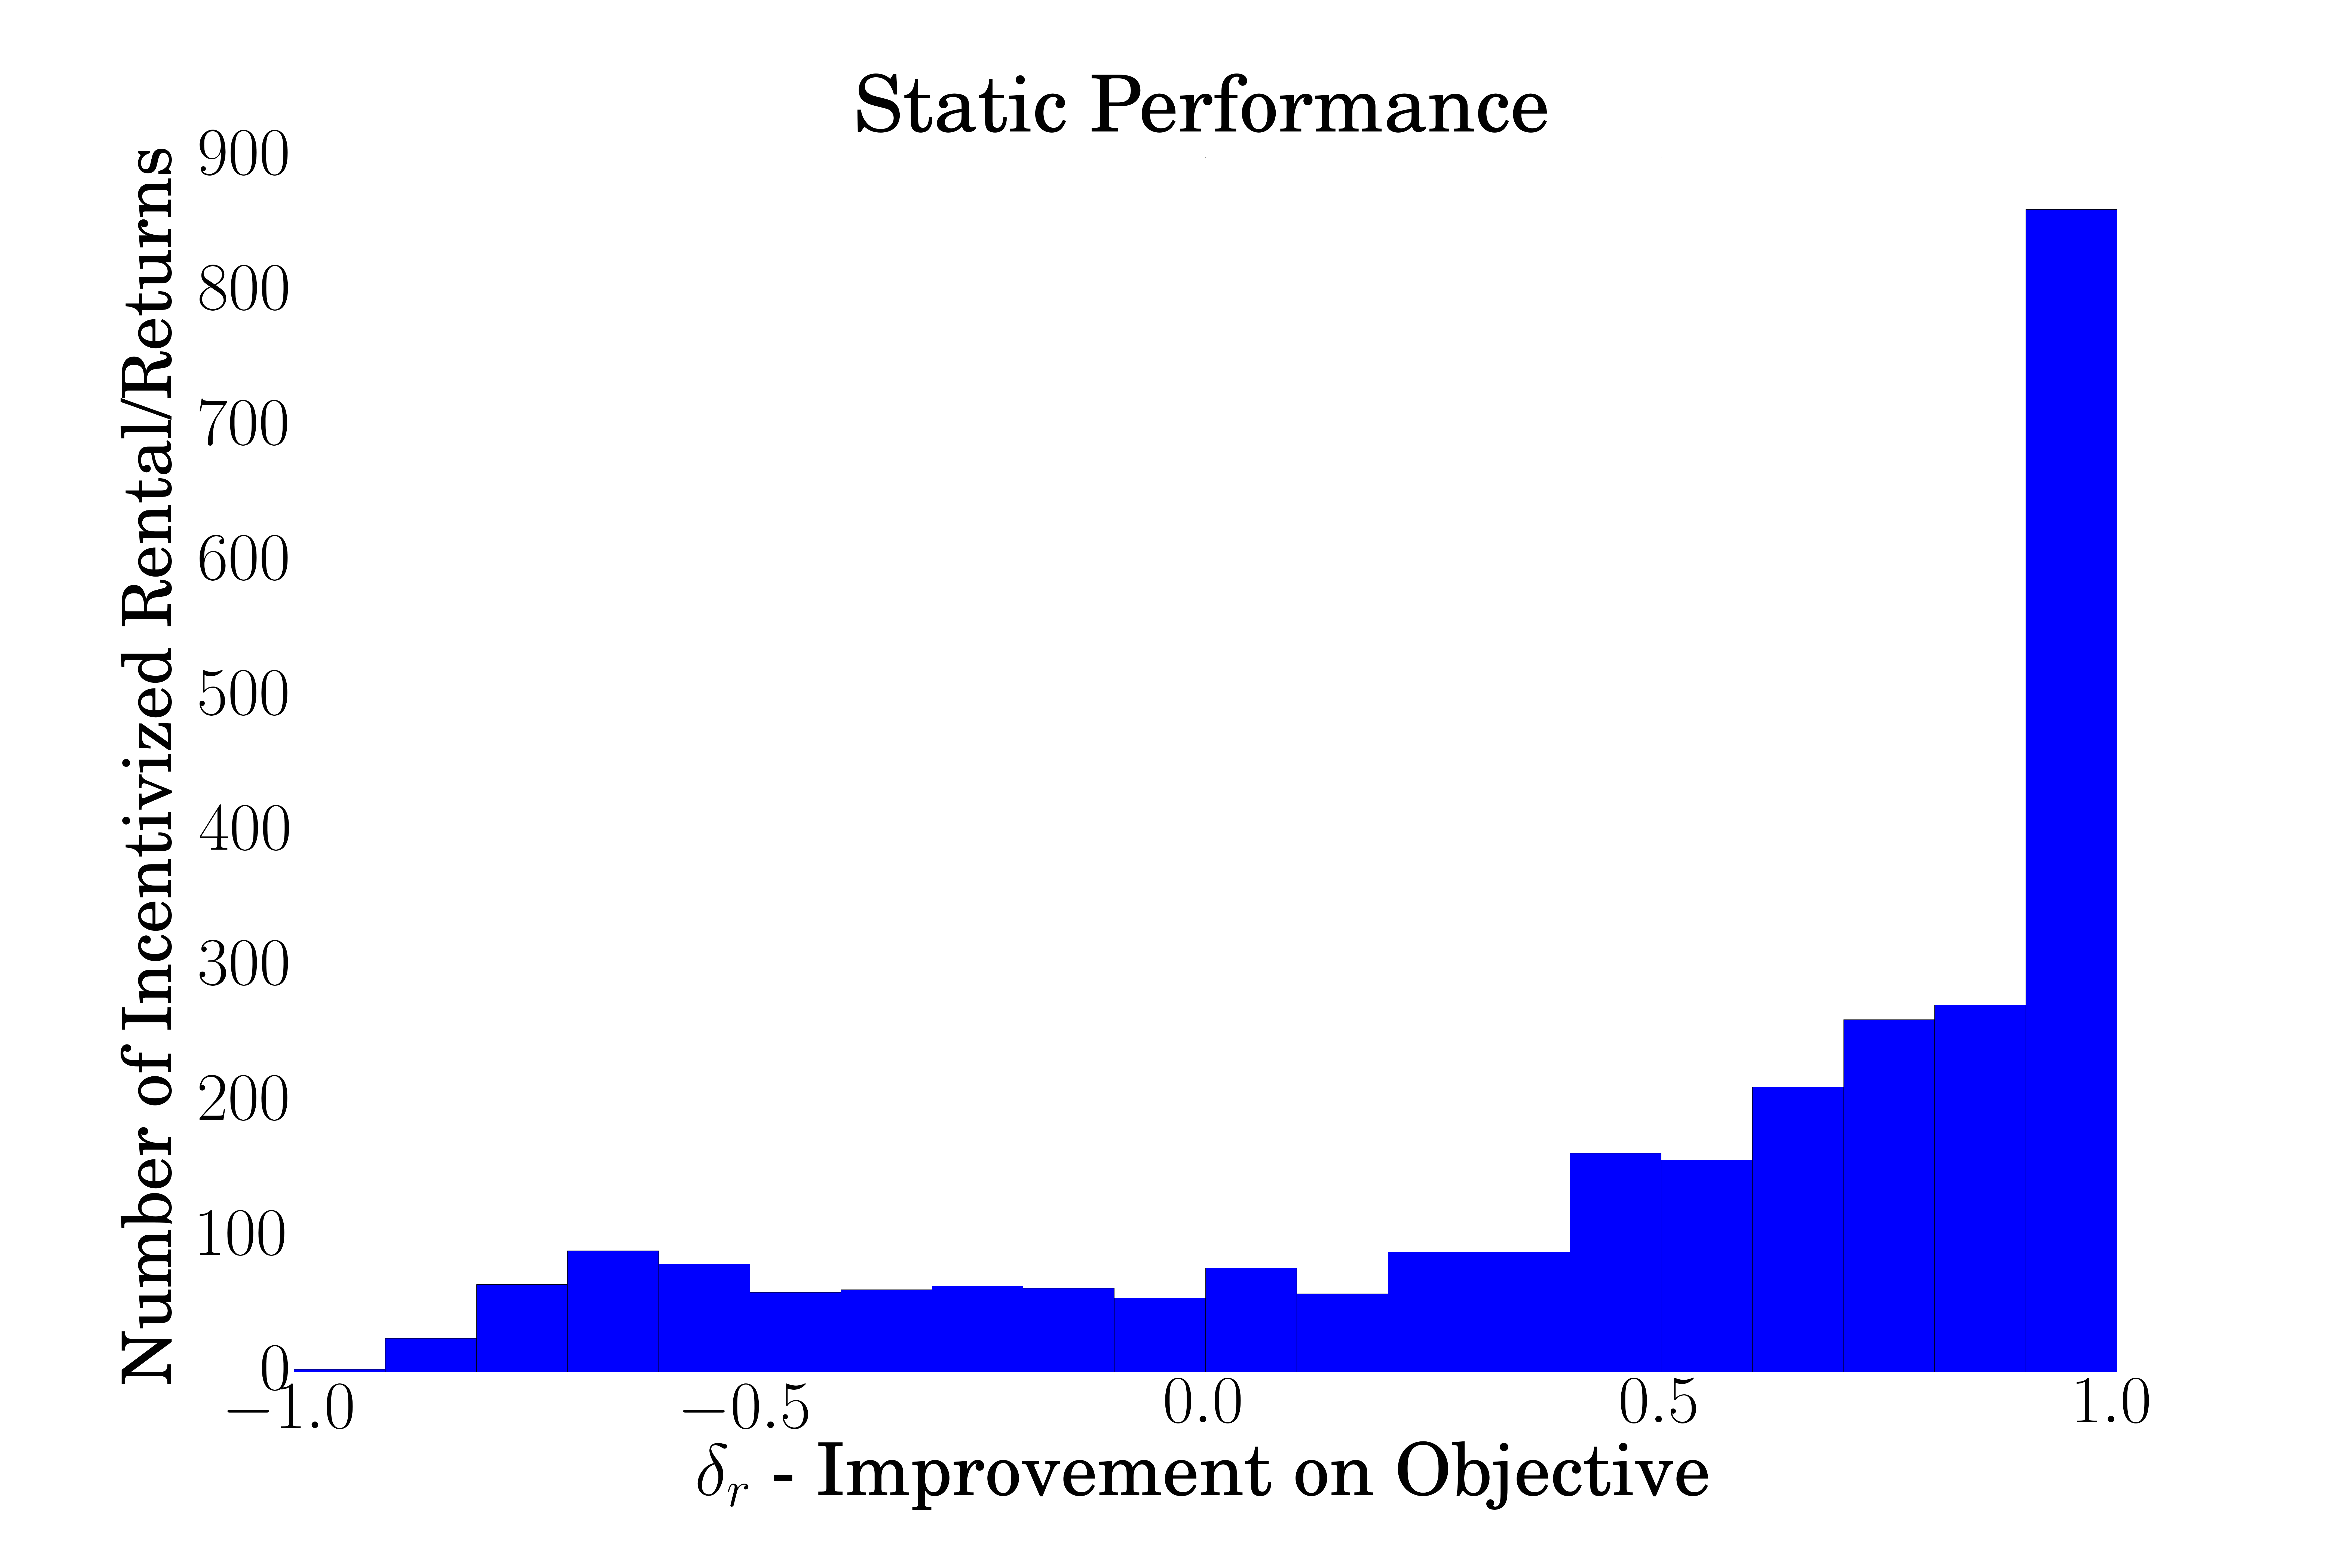
\includegraphics[width=.5\textwidth]{../SubmissionPlots/ActuallyUsed/Static_Performance_PM.png}
\caption{Static Policy's total number of incentivized trips, grouped by impact on objective ($\delta_r$) for the PM period.}
\label{fig:Static Performance}
\end{figure}


%Original text.
%This exemplifies the importance of a data-driven approach to improve the Bike Angels program. For example, even a rather simple policy with minimal overhead, such as Static Hindsight, significantly improves the efficiency of the incentives.

\subsubsection{Static Optimal Benchmark Performance}
The online policies have two advantages over the offline policies: the flexibility to adapt decisions with updated information and the flexibility to incentivize over periods that are not sub-intervals. Comparing the performance of the Static Optimal to the Dynamic policy helps us  distinguish between these two effects. More specifically, the benchmark operates with perfect information but is constrained to only incentivize over sub-intervals. %Thus if the benchmark performs near-optimal, it suggests subinterval incentives are reasonable, and vice versa.

In Table \ref{table:det} we do indeed observe Static Opt achieving a near optimal score of 0.98, which only slightly worsens with increased costs. This supports our assumption that it suffices to incentivize over a single sub-interval. However, Static Opt assumes perfect knowledge and still only matches the performance of Dynamic CC (60). In that sense, it also demonstrates the limitations of the best feasible offline policies.

\subsubsection{Online to Offline Policies}
Unsurprisingly, we find that the online policies outperform offline policies. As we transition from the maximally dynamic and online policy to the entirely static and offline policy, the decrease in performance occurs in a somewhat smooth way. % show an interesting smooth decrease in performance as we . If we imagine placing the policies on a dynamic/static spectrum, with Dynamic on one end and Static on the other, the results exemplify the continuous trade-offs between efficiency and simplicity as we move along the spectrum. Concrete examples of this trade-off in terms of the operator and user's experience is the following: with more dynamic online policies the incentives are more efficient; however, this comes at the cost of simplicity for the operator in terms of the increased IT set-up, and for the user in terms of the undesirable reduced predictability on where incentives will be given in the future. 

An interesting result in this context is the performance of the Dynamic CC (15) policy in Tables \ref{table:det} and \ref{table:stoch}, as it achieves optimal scores for all sets of parameters; this demonstrates that making decisions completely online/in real time is not necessary to obtain perfect efficiency.

On the other end of the spectrum from online to offline, the results of Table \ref{table:det} demonstrate that the offline policies Static Hindsight and Cluster Hindsight perform almost on par with the online Dynamic CC (120) policy, especially in the regime with low cost parameters; this points to the limited advantage of the simple online policies as the cost parameter increases. %This indicates that the benefits of an online policy with dynamic decision making is almost insignificant at this point of the dynamic/static spectrum.

\subsubsection{The Cost Parameter}
%New
In considering the relative performance change of policies with increasing cost parameters, we find that the offline policies are comparatively much worse at handling high cost parameters than the online policies. Intuitively, it might seem that the interval incentive restrictions of offline policies leads to this result. For example, imagine taking the original incentive interval with no cost parameter, and changing some of the positive-impact trips within the interval to become negative-impact trips (due to increase in cost). Then unless these trips all exist at the outer limits of the interval, these trips will "shatter" the incentive interval: either the offline policies give up on the positive-impact trips at the beginning or they give up on the positive-impact trips at the end or they include the negative-impact trips in the middle. Online policies on the other end can avoid this conundrum as they are not restricted to a single sub-interval. 

However, the performance of the Static Optimal benchmark in Table \ref{table:det} does not significantly degrade with high cost parameters. Thus, despite the interval restriction, the offline policies still have room to have better predictions yield improved performance.

In contrast, Figure \ref{fig: Dynamic CC 60 Policy} displays for the Dynamic CC (60) all incentivized trips with their time of day, their expected impact on future out-of-stock events, and for each one, the decision whether or not it is incentivized when run with 2 different cost parameters.% within nicely illustrates how the dynamic policies adapt to increased cost parameters. % shows the c of Dynamic CC 60 as cost parameters are increased from 0.0 to 0.3. The top scatter plot indicates for each incentivized trip, indexed by time of trip and $\delta_r$, whether it is included/excluded in the Dynamic CC 60 policy incentivization under a 0.0 cost parameter regime. The bottom plot is the same plot except when the cost parameter is increased to 0.3. 
The cost parameter is specified in each plot by the y-value of the horizontal line dividing the positive-impact trips (above the line) and negative-impact trips (below the line). As the cost parameter increases from 0.0 to 0.3, the policy excludes most trips having a $\delta_r$ value between that range, that it had previously included. Thereby, it manages to retain its near-optimal performance.



%The efficiency of online policies even with increasing cost parameters can be seen in the two scatter plots of Figure 4, that indicate which incentivized trips are included/excluded in the Dynamic CC 60 policy under low (0.0) and high (0.3) cost parameter regimes. The trips are indexed by time of day on the x-axis and $\delta_r$ value on the y-axis, and the cost parameter is specified by the y-value of the horizontal line dividing the positive-impact (above the line) and negative-impact (below the line) trips for the respective cost. The figure shows how the Dynamic CC 60 policy gracefully handles the increase in cost parameter from 0.0 to 0.3 by excluding most trips it had previously included with a $\delta_r$ value between that range.


\begin{figure}
\centering

 \begin{subfigure}{\textwidth}
 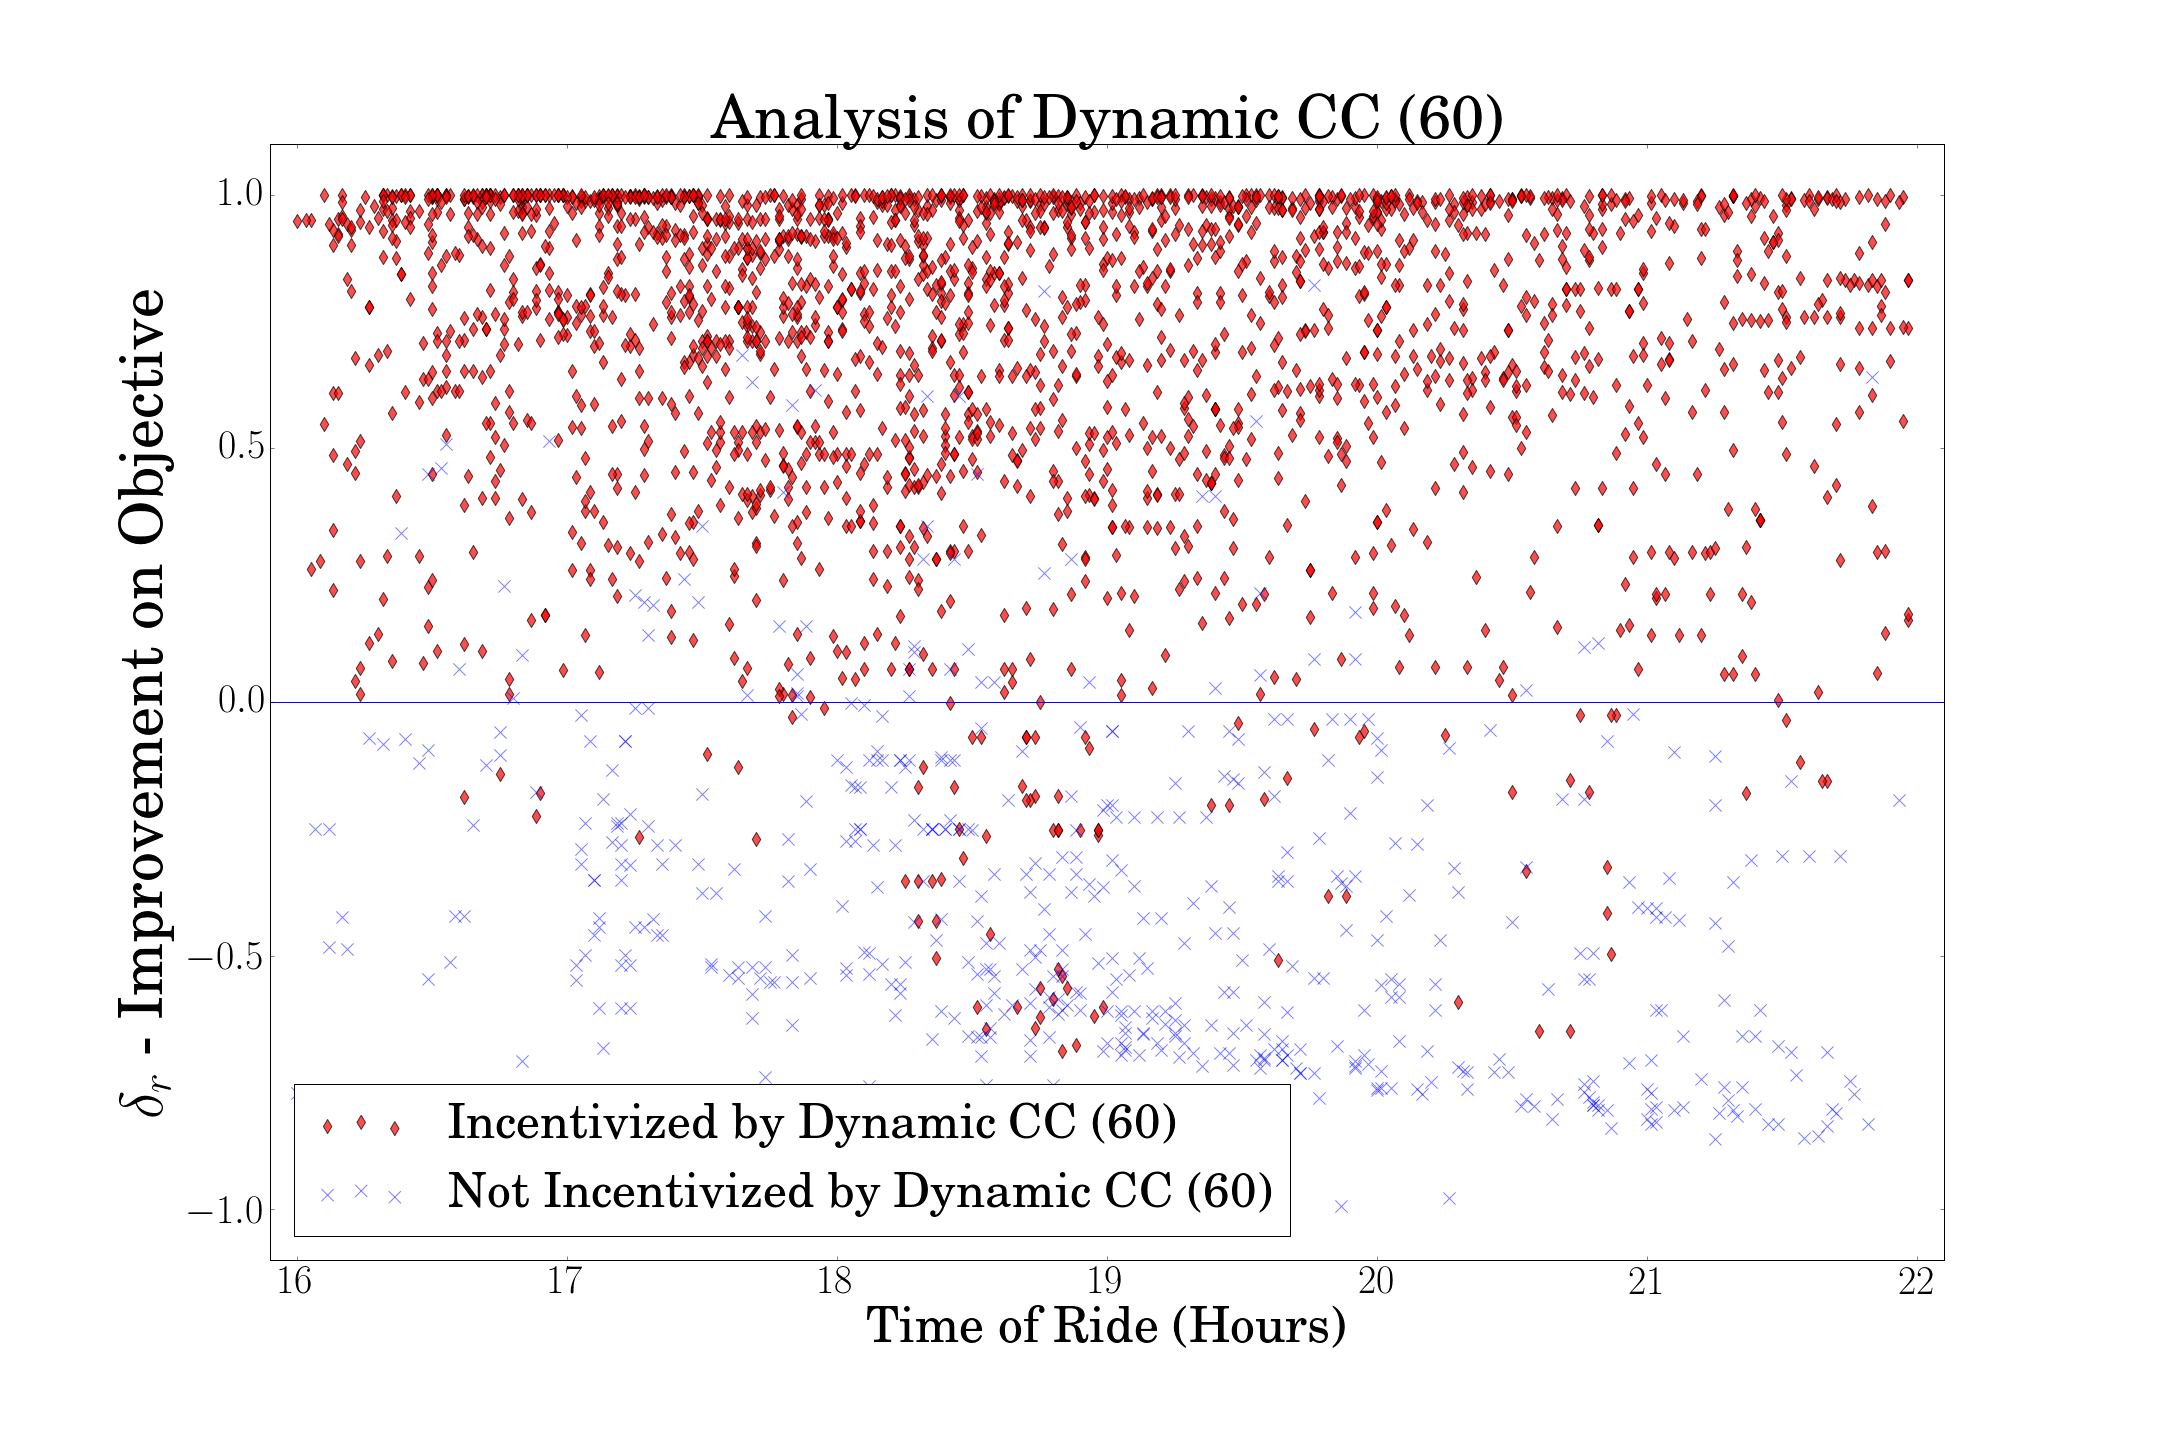
\includegraphics[width=.5\textwidth]{../SubmissionPlots/ActuallyUsed/scatter_60_0.png}
 \end{subfigure}
 \begin{subfigure}{\textwidth}
 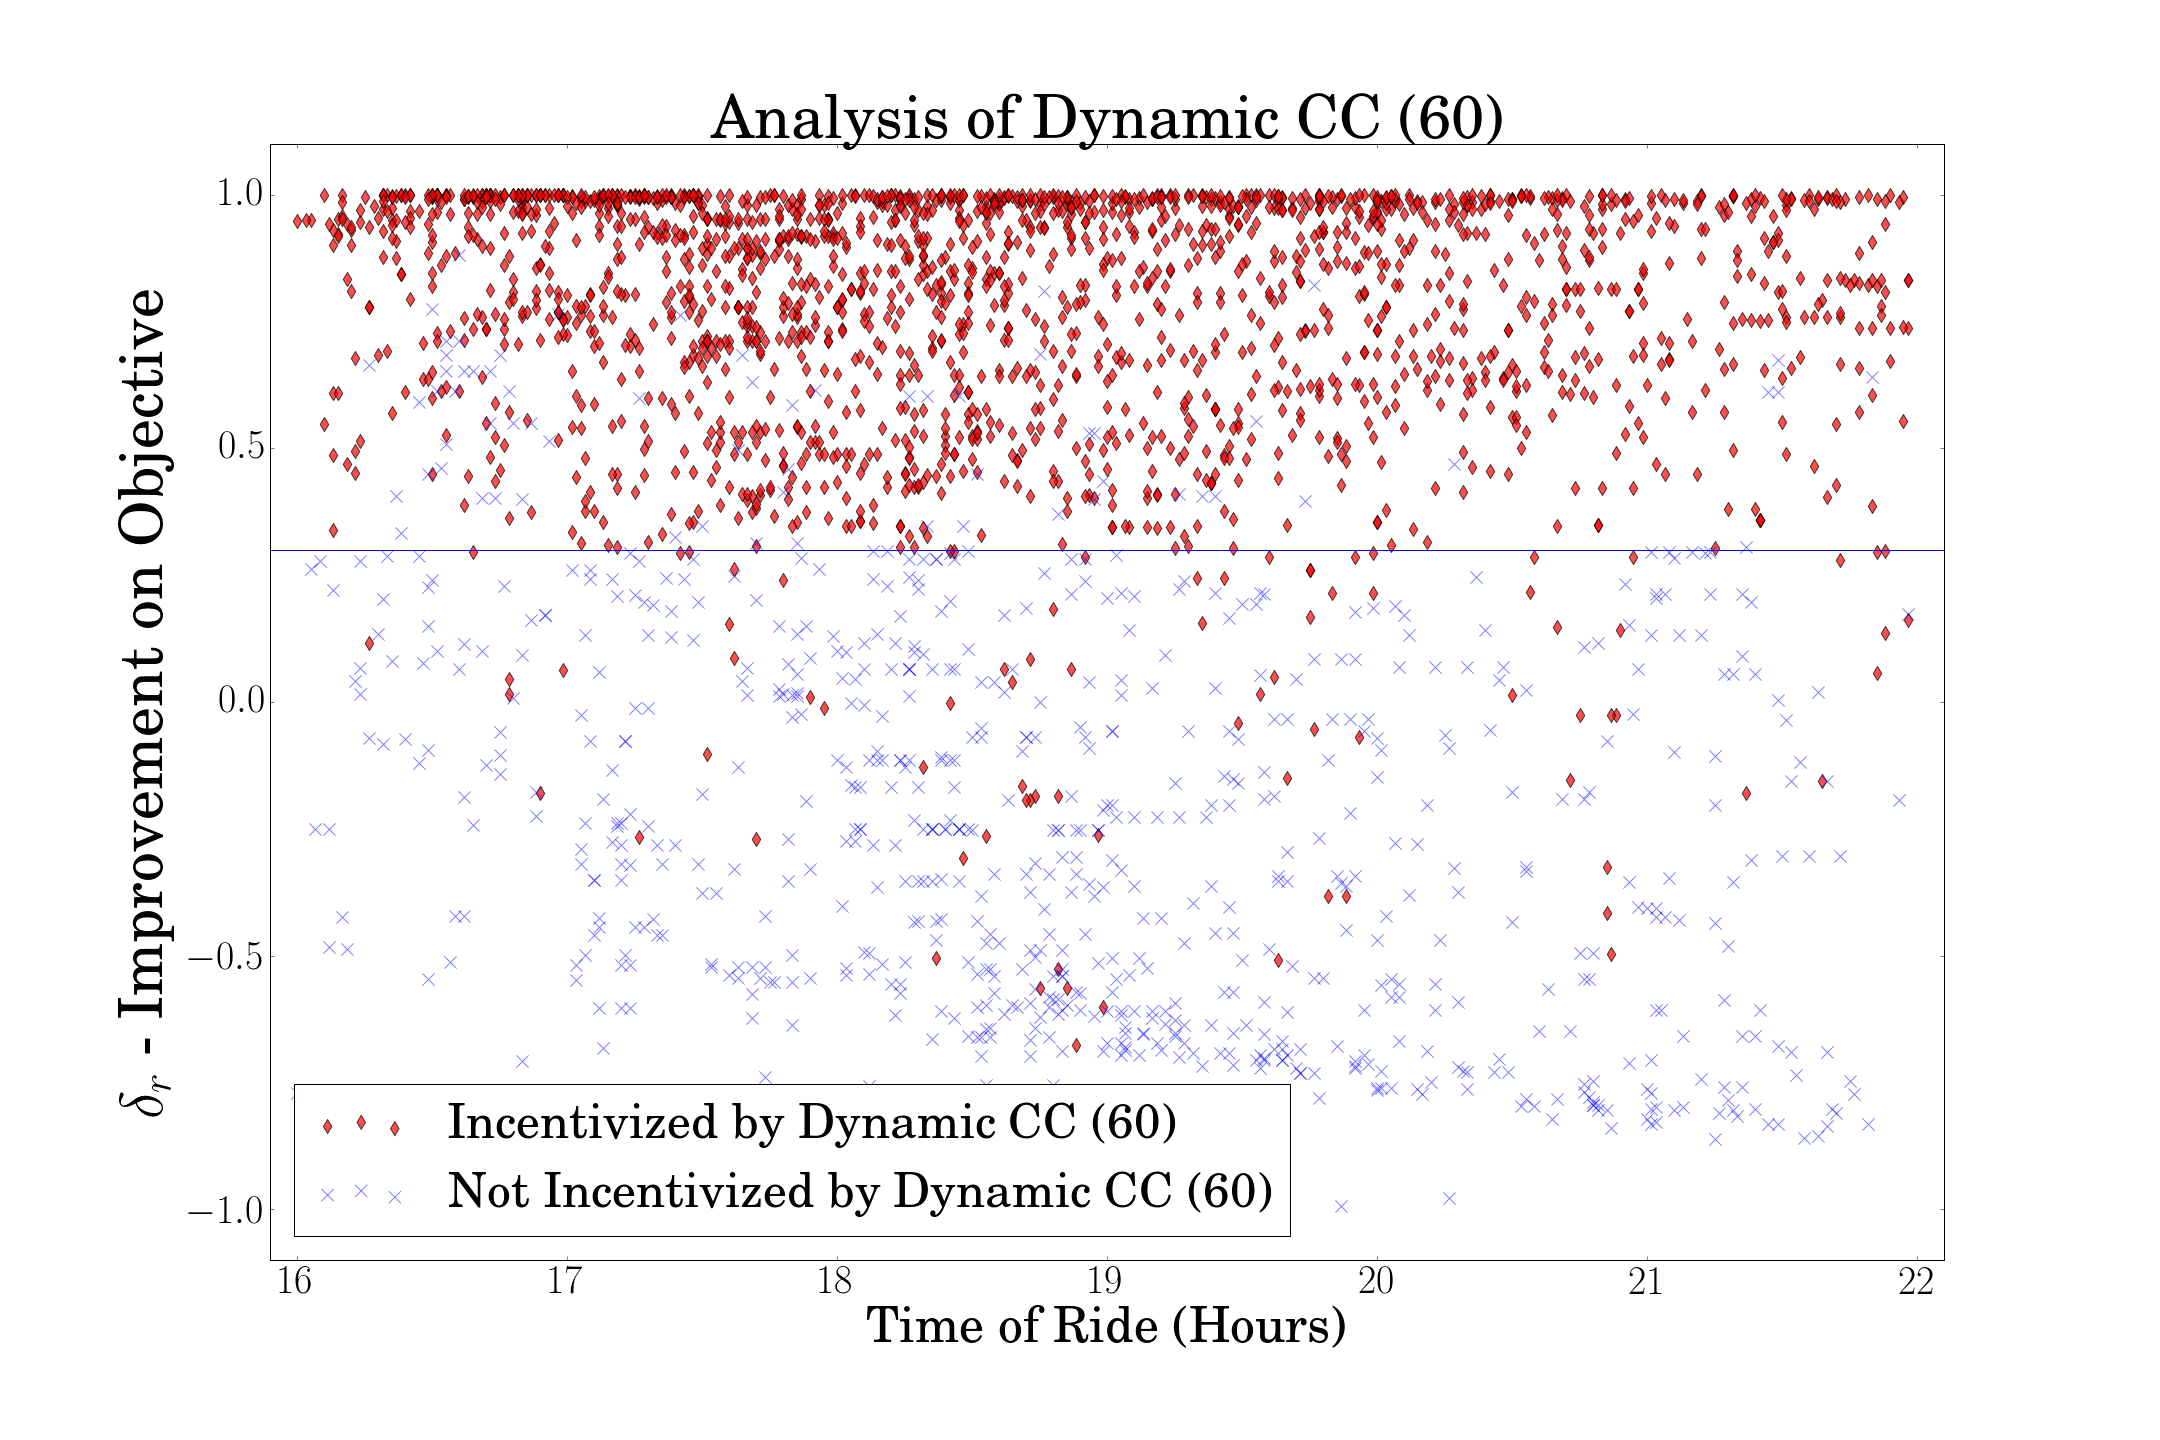
\includegraphics[width=.5\textwidth]{../SubmissionPlots/ActuallyUsed/scatter_60_3.png}
 \end{subfigure}
 
 \caption{Scatter plots of incentivized trips indicating which trips are included/excluded in Dynamic CC (60) incentivization policy, when cost parameter is 0.0 (top) and 0.3 (bottom).}

\label{fig: Dynamic CC 60 Policy}
\end{figure}


%Before
%In considering the relative performance change of policies with increasing cost parameters, we find that the offline policies are comparatively much worse at handling high cost parameters than the online policies. Intuitively, it might seem that the inherent interval incentive restrictions of offline policies leads to this result. For example, imagine taking the original incentive interval with no cost parameter, and changing some of the positive-impact trips within the interval to become negative-impact trips (due to increase in cost). Then unless these trips all exist at the outer limits of the interval, these trips will "shatter" the incentive interval: either the offline policies give up on the positive-impact trips at the beginning or they give up on the positive-impact trips at the end or they include the negative-impact trips in the middle. Online policies on the other end can avoid this conundrum as they are not restricted to a single sub-interval. However, the performance of the Static Optimal benchmark in Table \ref{table:det} does not significantly degrade with high cost parameters, indicating that even with the interval restriction, the offline policies still have room to have better predictions yield improved performance. %inability of offline policies to handle high cost parameters is due not only to the interval restriction, but also a characteristic of each offline policy and leaves room for improvement.

\subsubsection{AM and PM Periods}
Comparing the policy performances from the AM to PM period, we find there is a significant performance difference (i.e., all policies perform worse in the PM). However, in light of the results in Table 1, we see the relative performance order of the policies with each other is consistent. This indicates that the system behavior of Citi Bike is fundamentally more erratic in the afternoon, leading to all policies having a harder time predicting when to incentivize.

\subsection{Stochastic Evaluation}

In this section we highlight four noticeable differences between the results in Tables \ref{table:det} and \ref{table:stoch}.

\subsubsection{Limiting Cost Parameters}
When evaluating Stochastic performances we limit the cost parameters to only go as high as 0.2. This is because when incorporating the likelihood of trips into the $\delta_r$ calculations, the expected impact of a trip before subtracting the cost is much lower; in particular, it is easy to show that the impact of a single incentivized rental/return is at best a reduction of 1 in the number of out-of-stock events. But then, if for example the probability of a particular rental having been triggered by an incentive was 0.5, then even with an impact of 0.8, there would be no improvement with cost parameter 0.4.

\subsubsection{Relative Order}

The results in Table \ref{table:stoch} show that the same general trends  in relative performance order (most dynamic to most static) that hold for the deterministic results, also hold for the stochastic results. Likewise, the results indicate that the Static Optimal benchmark still performs near optimally in the stochastic setting.

A key difference between the deterministic and stochastic results is the sensitivity to cost parameters. In particular, except for the Dynamic CC policies parameterized with 15 and 30, all policies decrease significantly in performance with even small increases in the cost parameter. Intuitively, due to the newly introduced stochasticity, the expected impacts of all rides are reduced, and small changes in cost are still large, relative to the reduced impacts. 

\subsubsection{Advantage of Hindsight Policies}

Another interesting difference found between the deterministic and stochastic results is the relative performances of the Dynamic CC 60 and 120 policies compared to the Static Hindsight and Cluster Hindsight policies. Without stochasticity, the online policies dominated the offline policies in performance. However, when introducing stochasticity and for higher cost parameter regimes, the opposite seems to be true.  Intuitively this makes sense. The Dynamic CC X policies only consider the status of the station at the beginning of each X-minute interval, which includes the probability of an incentivized rental/return having occurred due to the incentive at that time (thus ignoring the differing probabilities existing within the X-minute interval). In contrast, the Static Hindsight and Cluster Hindsight policies actually incorporate all probabilities when computing the optimal incentive intervals in hindsight. 

\subsubsection{Static Policy}

Finally, from the stochastic results we see an even greater difference in performance between the baseline Static policy and all other policies (especially with increasing costs). The large differences again underline the performance improvements that can be obtained by transitioning from the Static policy to a data-driven policy.
  





\section{Conclusion}\label{sec:angel_conclusion}

We have proposed a number of data-driven policies to guide incentives for rebalancing in bike-sharing systems via crowdsourcing. While our analysis clearly displays the performance differences between these policies, the superior performance of the more dynamic policies comes with the cost of greater complexity for users and operators alike. % greater  difficulties for users and operators alike than the simpler ones.
%We have developed several policies for an incentive program like Bike Angels. 

%Beyond the policies described in the paper, we also tried two other offline policies: one based on a fluid model, similar to \cite{jianetal}, another based on a clustering approach that is more explicitly related to the user dissatisfaction functions. The fluid model performed very poorly (70-80\% of the optimal performance in the deterministic regimes), the clustering approach performed very consistently with around 85\% of the optimal policy. Noticeably, the latter did not degrade very much with increased cost parameters. We decided not to include them in the paper as they seemed dominated by the other offline policies in both simplicity and on efficiency.

There are other important considerations beyond their simplicity and performance. For example, when comparing the performance of the Static and Cluster Hindsight policies, it seems unclear at first glance what additional value the Cluster Hindsight policy provides, given that it relies on heavier machinery -- after all, they perform very similarly. However, the Static Hindsight policy can only be defined for stations for which the Static policy had been in place, whereas the Cluster Hindsight policy can be defined for other stations as well. Thus, in a way, each of the policies presented has its own advantage.

Most importantly, our analysis shows that slightly limiting the online fashion of decision-making only causes limited decreases in performance. On the academic side, this adds a data-driven analysis to a recent stream of literature in operations management that compares dynamic and static decision-making in similar applications. On the practical side, our analysis led to Citi 	Bike adopting a version of the Dynamic CC (30) policy in 2017. 

%Bike Angels has developed into a popular progra

%Items to cover:

%Cluster Hindsight is useful for adding new stations (as opposed to Static Hindsight)

%Fluid policy we tried, but it's bad.

%Bike Angels now runs, effectively, on Dynamic CC (30)

%Contribution: data-based approach to the fundamental question about online/offline decision-making with a particular application in sustainable transportation


%Finally, the results indicate that Cluster Hindsight and the much simpler Static Hindsight policy perform similarly. Considering the value of simplicity in policies, one might question why the more complicated policy is needed at all. However, the Cluster Hindsight policy is important because it provides the additional benefits of being able to automatically identify stations in need of incentivization as well as provide reasonable incentive intervals for such stations. This is because the clustering of stations performed in the policy does not rely on any past incentive data, allowing any new stations to be included into the clustering and be considered for incentivization. This can prove vital for bike-sharing systems as system usage grows, as the policy provides a mechanism to automatically decide which stations to incentivize and when. 

%\section{Start-Stop Policies in Fluid Models}%\label{sec:fluid}
%The focus on incentive schemes over intervals is motivated by the theorem we present in this section;  intuitively, the theorem gives conditions under which it is optimal, in the fluid model, to only incentivize during at most two intervals of the day (one for rentals, one for returns). We first state the condition under which the above fails and then prove that it otherwise holds. Next, we evaluate through data the extent to which the condition in the theorem holds true in the Citi Bike system. Finally, we use extensive simulations to compare the result in the fluid setting with that in continuous-time Markov chain models.

\subsection{Theorem} 
\label{ssec:theorem}


\textbf{Asymetric Condition.} Suppose we are given a capacity $K$, an initial number of bikes $b$, rates $\mu(t)$ and $\lambda(t)$ for rentals and returns without incentivizing and corresponding rates $\hat{\mu}(t)$ and $\hat{\lambda}(t)$ for rentals and returns with incentivizing. Then, the \emph{asymetric condition} holds unless either there exist $t_1<t_2<t_3<t_4<t_5<t_6$ such that
\[
\min\{
b+\int_{t_1}^{t_2} \lambda(t)-\mu(t)dt,
\int_{t_3}^{t_4} \mu(t)-\lambda(t)dt,
\int_{t_5}^{t_6} \lambda(t)-\mu(t)dt
\}
\geq K
\]
or there exist $t_1<t_2<t_3<t_4<t_5<t_6$ such that
\[
\min\{
K-b+\int_{t_1}^{t_2} \mu(t)-\lambda(t)dt,
\int_{t_3}^{t_4} \lambda(t)-\mu(t)dt,
\int_{t_5}^{t_6} \mu(t)-\lambda(t)dt
\}
\geq K.
\]

\textbf{Incentives help weakly.} We assume that (i) incentivizing rentals (return) at a station yields a higher rate of rentals (returns) than not doing so and (ii) it does not change the sign of the net-flow at the station, that is, a station that loses bikes (on average) continues to do so (on average) even with incentives.  $(\hat{\mu}(t)-\lambda(t))(\mu(t)-\lambda(t))> 0$ and $(\mu(t)-\hat{\lambda}(t))(\mu(t)-\lambda(t))> 0$.


\textbf{Lemma.}
%\begin{lemma}
Suppose for given data that both conditions hold. Then, in the fluid model, there exist $T_s, T_S, T_s',T_S'$ such that it is optimal to incentivize rentals during $(T_s,T_S)$ and returns during $(T_s', T_S')$.
%\end{lemma}

\emph{Lemma.}
%\begin{proof}
We argue by contradiction. Consider a set of intervals $(s_1,S_1),\ldots,(s_k,S_k)$ such that incentivizing rentals during $(s_j,S_j)$ for even $j$ and incentivizing returns during $(s_j,S_j)$ for odd $j$ (i) is  optimal, (ii) subject to (i) $k$ is minimized, (iii) subject to (i) and (ii) $S_2-s_1$ is minimized, and (iv) subject to (i)-(iii) $S_3-s_2$ is minimized. Notice by symmetry of rentals and returns that flipping the odd and even intervals in (i) does not affect the argument. Further, the case that it is optimal to incentivize returns (rentals) in two consecutive intervals is excluded by the two conditions combined with the intervals being chosen such that $k$ is minimized. We aim to show that the above lead to a contradiction with the asymmetric condition.

Notice that (iii) implies in particular that for any $\epsilon, \epsilon'>0$ it must be strictly worse to incentivize returns from $s_1+\epsilon$ to $S_1+\epsilon'$ instead of $s_1$ to $S_1$; by the assumption that incentives help weakly, there must exist arbitrarily small such $\epsilon,\epsilon'$ such that incentivizing returns from $s_1+\epsilon$ to $S_1+\epsilon'$ gives the same total increase in returns as from $s_1$ to $S_1$, yet decreases by $\epsilon$ the difference between the end of the second and the beginning of the first interval. By (iii), this implies that doing so would give a strictly smaller objective. We claim that this also implies that the fluid must be empty at least once at a time $T\in(s_1,S_1)$. Indeed, suppose it were the case that the fluid never hits 0 in $[s_1,S_1]$. If it never hits $K$ either, then there  exists sufficiently small $\epsilon'$ such that no cost is incurred in $[s_1,S_1+\epsilon']$ and we could set  $\epsilon,\epsilon'>0$ such that incentivizing returns from $s_1+\epsilon$ to $S_1+\epsilon'$ gives the same fluid level of bikes at time $S_1+\epsilon'$ we would have when incentivizing in $(s_1,S_1)$ -- a contradiction to (ii). Else, it does hit $K$ but does not incur a cost at that point (not incentivizing returns at that point would be better, so incurring a cost would violate (i)); in that case, there is again no censoring, so incentivizing returns in $(s_1+\epsilon,S_1+\epsilon')$ can be no worse. 

TODO this last part of the argument is unclear

Thus, it must be the case that the fluid model with the incentives set by the policy is empty at a time $T\in(s_1,S_1)$. In particular, this implies that with $t_1=0, t_2=T$ it is the case that $\int_{t_1}^{t_2} \mu(t)-\lambda(t)dt\geq b$.

By the same reas

%By the same reasoning as before, there must be a time $T'\in(s_2,S_2)$ when the fluid model must have the station be full, implying that with $t_3 = T, t_4=T'$ we have $\int_{t_3}^{t_4}\lambda(t)-\mu(t)\geq K$.

Again with the same reasoning, we find that there is a time $T''\in(s_3,S_3)$ where the station must be empty, so with $t_5=T'$ and $t_6=T''$ we have $\int_{t_5}^{t_6} \mu(t)-\lambda(t)dt\geq K$. As such, the $t_1,\ldots,t_6$ contradict the asymmetric condition and thus imply the lemma statement.

%Thus, with there must exist two intervals that minimize
 
%\end{proof}


\subsection{Verification of Condition}

\subsection{Fluid vs. Continuous-time Markov chain}



% BALANCE COLUMNS
\balance{}

% REFERENCES FORMAT
% References must be the same font size as other body text.
\bibliographystyle{SIGCHI-Reference-Format}
\bibliography{references}

\end{document}

%%% Local Variables:
%%% mode: latex
%%% TeX-master: t
%%% End:
